\chapter{Results}
\label{ch:results}

	\section{Deforestation}
	\label{sec:results_deforestation}

		\subsection{Forest definition}
		\label{subsec:results_forest_definition}
		%TODO Holm correction to one-sided tables
		%TODO switch image all regions to global, americas to south america
			Our goal is to determine at which canopy cover density the agreement between \ac{GL30} and \ac{GFC} tree cover is greatest to receive the subsequent \ac{PDD} for stable \ac{LC} transitions introduced by anthropogenic causes. This process should ensure that we keep the largest number of tree cover loss samples from the \ac{GFC} dataset while harmonizing the tree cover definition between both layers. We applied the \ac{JI} to determine the similarity between each tile pair from our \ac{AISM}. The \ac{JI} computation is grouped by the continental regions Americas (82 tiles), Asia (86 tiles), and Africa (101 tiles). We determined the similarity for the following canopy density intervals: $(0, 100]$, $(10, 100]$, $(20, 100]$, and $(30, 100]$. Later we excluded all tiles with a initial \ac{JI} (canopy density intervall $(0,100]$) from our analysis because these tile pair does not contain any tree cover. We excluded 6, 9, and 15 tiles for Americas, Asia and Africa, respectively. To determine the canopy density interval where the agreement is at maximum we applied the non-parametric tests Wilcoxon signed-rank test and Wilcoxon rank-sum test. Both of the tests are performed as a one- and two-sided to deduce, if there is a difference in agreement (equality) and which direction (less or greater) has this difference. To address the higher probability of family-wise error rate in multiple comparisons we applied the Holm correction. We applied continental and global testing to deduce regional differences and to determine the optimum for our subsequent \ac{PDD} predictions. Further, we compared the tree cover agreement of the three continental regions. Our initial hypothesis was that the tree cover agreement is at its maximum within the canopy density interval of $(30,100]$ for the entire study extent. We assumed that for the Americas and Asia the best results could be achieved with the same canopy density threshold. For Africa we assumed that the highest agreement could be achieved within the interval of $(10,100]$ because this region comprises a higher frequency of sparse woodland cover. The following paragraphs present our results for the three regions in the following order: Americas, Asia and Africa. The last paragraph discusses the results for the entire study extent and determines which canopy density we used for the following \ac{PDD} prediction.

			For Americas, Asia and Africa as well the entire study extent figure \ref{fig:jaccard} shows the distribution of the computed \acp{JI} for all tile pairs within the canopy density intervals. The x-axis are the different canopy density intervals where the label $JI_0$ accounts for $(0,100]$, $JI_1$ $(10,100]$, $JI_2$ $(20,100]$, and $JI_3$ $(30,100]$, respectively. The y-axis is the corresponding \ac{JI} between 0 and 1 where 0 highlights a complete disagreement and 1 a full agreement. The sample mean is labelled by a red cross and the boxes comprises the $Q_1$ (25 \%), $Q_2$ (50 \%), and $Q_3$ (75 \%) sample interval, respectively. For the Americas the sample mean does not change significantly within the four canopy density experiments. It is approximately 0.62 while sample median decreases from 0.68 to 0.66 from the interval class to the last. The upper 25 \% of the first experiment interval have a tree cover similarity ranging between approximately 0.8 and 1. This holds true over the other three experiments while only the maximum similarity slightly increases from 0.9787 to 0.9798. The figure \ref{fig:jaccard_americas_appendix} in the appendix suggests, that exclusions of canopy densities smaller than 11 increases slightly the tree cover agreement of the upper 25 \% but the exclusion of higher canopy density provides no benefit. This can be explained by the fact that the upper percentile already contain samples with a high tree cover agreement and it is to assume that only a small number of pixels have canopy density smaller than 30. Therefore, the interval change has only a small impact on this samples. For the first two canopy density intervals the range of the lower 25 \% percentile is between approximately 0.0003 and 0.45. Whereas the range increases from 0.0 to 0.5 for the last two interval classes. The figure \ref{fig:jaccard_americas_appendix} reveals a strong regional dependency of tree cover agreement within different canopy density classes of the lower percentiles. Whereas samples from the northern hemisphere show a decline in agreement the samples of the southern hemisphere show a increase of agreement. The strong up-shift of the southern samples within the last two intervals increases the range of lower percentile. This suggests in general that samples with low tree cover agreement benefit by the exclusion of lower canopy densities. The mobility of the samples within the $Q_1$ and $Q_3$ percentile show no general trend. For the first two experiments it ranges between 0.5 and 0.8 and for the last two it shows a small decline in $IQR$. This suggests that tiles within this group could benefit from a local optimisation of canopy density exclusion. We applied a Wilcoxon signed-rank test to deduce which canopy density class yields the highest tree cover agreement overall samples in the Americas. Table \ref{tab:wilcoxontwosided_regions} shows the results for the two-sided test and table \ref{tab:wilcoxontwosided_regions} for the one-sided test. The two-sided test reveals that only the similarity distribution between $JI_0$ and $JI_1$ is significantly different ($p<0.01$), while the comparison of the other distributions suggest that they are equal. The directional test of $JI_0$ and $JI_1$ suggests that the regional tree cover agreement is significantly greater ($p<0.005$) if canopy densities smaller than 10 are excluded. Additionally the table shows that $JI_2$ is significantly greater (p<0.05) than $JI_0$ but the comparison between $JI_1$ and $JI_2$ shows no significant difference. Therefore both tests confirm a strong regional or single tile agreement component. The directional test does not confirm that the distribution if $JI_1$ is significantly greater than $JI_2$ and $JI_3$. As the results of our experiments suggests is the tree cover agreement between \ac{GL30} and \ac{GFC} at canopy densities greater than 10 highest within the entire topical Americas. In case of local studies or for smaller extents the canopy density should be selected by a single tile approach to optimise the tree cover agreement by maximising the number of data points of the \ac{GFC} dataset.
			\begin{figure}[ht]
				\centering
				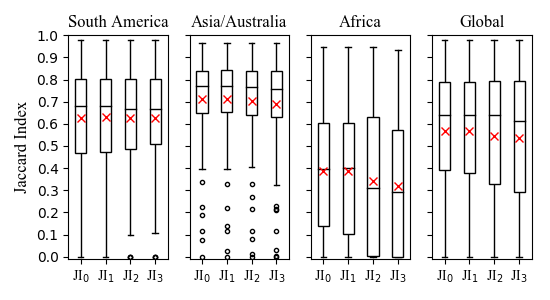
\includegraphics[scale=.91]{img/jaccard}
				\caption[Tree cover similarity distribution of the continental regions]{\textbf{Tree cover similarity distribution over the continental regions:} This boxplot shows the distribution of computed Jaccard Index for each raster image tile pair of GlobeLand30 and Global Forest Change tree cover from 2000. The labels $JI_0$, $JI_1$, $JI_2$, and $JI_3$ on the x-axis account for the canopy density classes (0,100], (10,100], (20,100], and (30,100], respectively. The y-axis is the computed Jaccard Index for the corresponding raster image pair, where 0 is a total disagreement and 1 a total agreement. Red crosses within the $Q_{25}$, $Q_{50}$, and $Q_{75}$ boxes highlight the sample mean. Whiskers are 1.5 times the $IQR$.}
				\label{fig:jaccard}
			\end{figure}
			\begin{table}[ht]
				\centering
				\caption[Regional two-sided Wilcoxon signed-rank test]{\textbf{Regional two-sided Wilcoxon signed-rank test:} This table shows, regional differences in the tree cover agreement by considering different canopy densities between GlobeLand30 and Global Forest Change at 2000. The classes $JI_0$, $JI_1$, $JI_2$, and $JI_3$ as row and column headings account for the canopy density classes (0,100], (10,100], (20,100], and (30,100], respectively. The test hypothesis is H$_0$: $X_1=X_2$ where $X_1$ is the column $JI_n$ class and $X_2$ the row $JI_n$ class. The significance is indicated by $p^{*}<0.05$, $p^{**}<0.02$, and $p^{***}<0.01$.}
				\label{tab:wilcoxontwosided_regions}
				\begin{tabular}{llllllllll}
					\hline
					& \multicolumn{3}{|c}{Americas} & \multicolumn{3}{|c|}{Asia} & \multicolumn{3}{c|}{Africa} \\
					Cls & JI$_0$ & JI$_1$ & JI$_2$ & JI$_0$ & JI$_1$ & JI$_2$ & JI$_0$ & JI$_1$ & JI$_2$ \\\hline
					JI$_1$ & .00$^{***}$ & - & - & .71 & - & - & .22 & - & - \\
					JI$_2$ & .30 & 1. & - & .00$^{***}$ & .00$^{***}$ & - & .09 & .09  & - \\
					JI$_3$ & .64 & 1. & 1. & .00$^{***}$ & .00$^{***}$ & .00$^{***}$ & .00$^{***}$ & .00$^{***}$ & .00$^{***}$ \\\hline
				\end{tabular}
			\end{table}
			\begin{table}[ht]
				\centering
				\caption[Regional one-sided Wilcoxon signed-rank test]{\textbf{Regional one-sided Wilcoxon signed-rank test:} This table shows, the direction of regional differences in the tree cover agreement by considering different canopy densities between GlobeLand30 and Global Forest Change at 2000. The classes $JI_0$, $JI_1$, $JI_2$, and $JI_3$ as row and column headings account for the canopy density classes (0,100], (10,100], (20,100], and (30,100], respectively. The test hypothesis is H$_0$: $X_1\leq X_2$ and H$_0$: $X_2\geq X_1$ where $X_1$ is the column $JI_n$ class and $X_2$ the row $JI_n$ class. The significance is indicated by $p^{*}<0.05$, $p^{**}<0.025$, $p^{***}<0.01$, and $p^{\dagger}<0.005$.}
				\label{tab:wilcoxononesided_regions}
				\begin{tabular}{lllllllllllll}
					\hline
					& \multicolumn{4}{|c}{Americas} & \multicolumn{4}{|c|}{Asia} & \multicolumn{4}{c|}{Africa} \\
					Cls & JI$_0$ & JI$_1$ & JI$_2$ & JI$_3$ & JI$_0$ & JI$_1$ & JI$_2$ & JI$_3$ & JI$_0$ & JI$_1$ & JI$_2$ & JI$_3$ \\\hline
					JI$_0$ & - & .00$^{\dagger}$ & .03$^{*}$ & .08 & - & .64 & 1. & 1. & - & .11 & .98 & 1. \\
					JI$_1$ & 1. & - & .18 & .25 & .36 & - & 1. & 1. & .89 & - & .99 & 1. \\
					JI$_2$ & .97 & .82 & - & .30 & .00$^{\dagger}$ & .00$^{\dagger}$ & - & 1. & .02$^{**}$ & .01$^{**}$ & - & 1. \\
					JI$_3$ & .92 & .75 & .70 & - & .00$^{\dagger}$ & .00$^{\dagger}$ & .00$^{\dagger}$ & - & .00$^{\dagger}$ & .00$^{\dagger}$ & .00$^{\dagger}$ & - \\\hline
				\end{tabular}
			\end{table}

			For Asia/Australia, the sample mean scatters around 0.7 as the red crosses in figure \ref{fig:jaccard} suggest. The sample mean decreases slightly at higher canopy density intervals. Further, the median is approximately 0.8 by showing a slight decrease at higher canopy density intervals too. The range of the upper percentiles for all experiments groups is between approximately 0.85 and 0.96 while the maximum agreement decreases slightly from 0.9654 to 0.9634. Figure \ref{fig:jaccard_asia_appendix} in the appendix, reveals that in general the tree cover agreement increases if canopy densities below 10 \% are excluded but the exclusion of densities above 20 \% reverts this. For Asia the lower percentile ranges between approximately 0 and 0.65 while most of the samples show a decline in tree cover agreement if canopy densities above 20 are excluded. Within the $Q_1,3$ percentile a per tile relationship is detectable. The range of this percentile is between 0.65 and 0.85 for the first two classes $JI_0$ and $JI_1$ while the range increases for the last two experiments. As mentioned no clear trend is observable some of the samples benefit if the considered canopy density interval is increased till 30 \% and some show a decrease in agreement if the canopy density is lift over 10 \%. The two-sided Wilcoxon test in table \ref{tab:wilcoxontwosided_regions} reveals that the similarity distribution is significantly different (p<0.01) between each experiment group except the pair of $JI_1$ and $JI_0$. The directional test in table \ref{tab:wilcoxononesided_regions} reveals that the tree cover agreement distributions of $JI_2$ and $JI_3$ are significantly smaller than $JI_0$ and $JI_1$ (p<0.005). Further this results show that the distributions of $JI_0$ and $JI_1$ have no directional differences. This could be explained by a regional or tile-wise agreement component. While some of the tiles show strong increase in similarity if canopy density is set to 10 \%, others show a decrease. A more detailed analysis could be performed by applying a smaller canopy density step-size. For studies targeting the region Asia the results of the directional tests suggest to use all data from \ac{GFC} within the canopy density interval of $(0,100]$. While the figure \ref{fig:jaccard_asia_appendix} suggests to include all data form the interval $(10,100]$.

			\note{Africa (review):} As figure \ref{fig:jaccard} for Africa suggests is the similarity distribution mobility of the samples in Africa at highest. The first two similarity distributions have an comparable mean and median at 0.38 and 0.4. The last two classes show a strong decline in mean and median to approximately 0.33 and 0.3. The mobility of the upper 25 percent of the first two canopy density classes is already quite strong as figure appendix suggests. While the iqr range for $JI_0$ is between 0.15 and 0.6 the range increases for the second $JI_1$ by connecting to more agreement downwards trend. The tile pairs in africa are characterized by 17 (approx. 20 percent) where the tree cover agreement is smaller than 0.1. 11 of these tiles have already a agreement of 0.0 when the first canopy density is excluded. These trend continues as more canopy density is excluded as more samples have a agreement of 0.0. This explains the high iqr range for the canopy densities exclusion greater than 10 percent. At $JI_3$ already two fifth (42 percent) of the samples have an tree cover agreement lower than 0.1. The two sided wilcoxon test shows that the distribution of $JI_2$ and $JI_3$ significantly differs (p<0.05 and p<0.01). As the table suggest is the distribution of $JI_0$ and $JI_1$ nearly the same. The one sided test reveals that reducing the canopy density below 10 percent decreases the tree cover agreement between sample distributions. For $JI_0$ and the $JI_1$ the test reveals that no clear trend is detectable. Appendix figure shows that some samples benefit from the exclusion of canopy density and as mentioned some samples show a strong decrease in tree cover similarity. As the data shows is the regional dependency of tree cover agreement at largest. To maximize the similarity on continental level for africa it should the entire data range of Global Forest Change should be slected. It could also be also a solution to select canopy densities in the interval 10 to 100 but here the trade is to have tiles where no tree cover agreement is detectable.

			\note{Comparison between regions (review):} Table appendix shows that Asia has the highest tree cover similarity distribution over all regions within all tested canopy classes followed by the Americas for GlobeLand30 and Hansen 2000. Africa has the poorest tree cover agreement within our tested regions. As discussed in the previous paragraphs the reason could be that Americas and Asia have mainly core tropical forest zones where the forest cover is dense and the canopy density is above 30 percent. This can be highlighted by section tropical deforestation and the shown tree cover maps. Africa in comparison to Asia and Americas has large zones where the tree cover is high but the canopy density is low also described by the term sparse woodland. As it looks these sparse woodlands compete the forest detection methods of both datasets. This fact could lead within the hansen dataset to ghost deforestation because it is hard to detect sparse woodland it could be the annual deforestation does not detect it as forest and it is recognized as deforestation. Therefore in africa the rationality of tree cover agreement must be considered during preparation and validation of studies. Also it is to suggest to optimize tree cover agreement on regional scale and not over the entire continent. Overall regions the upper 25 percent of the samples benefit or shown only small changes if the canopy density is increased.

			On the far right of figure \ref{fig:jaccard} the tree cover agreement of the entire study extent is presented. The sample mean and median differ between the first two experiment groups and the last two groups. For the first two groups the mean and median account for 0.56 and 0.63, respectively. The last two experiment groups show a decline to 0.53 and 0.53 for mean and median. For the upper percentile the same statement as for the regions holds true. In general, the samples with high tree cover agreement benefit from the exclusion of lower canopy densities. The lower percentile shows strong regional or tile-wise tree agreement dependencies. If we consider the entire sample range the mid percentile steadily increases its range from 0.4 to 0.8 till 0.3 to 0.8. As mentioned in the regional analysis, this percentile is characterized by inhomogeneous changes of tree cover agreement by the step-wise change of the canopy density. In general the trend points downwards as the decrease in median and the range increase show. The results of the two-sided Wilcoxon test in table \ref{tab:wilcoxontwosided_all} show a significant difference in distribution (p<0.02 and p<0.01) between each experiment group except $JI_0$ and $JI_2$ where the similarity distribution could be the same. Table \ref{tab:wilcoxononesided_all} highlights the directional component of these distribution differences. At a global scale the tree cover agreement is at its maximum if we set the canopy density interval to $(10,100]$. The second experiment group $JI_1$ is significantly greater than $JI_0$ (p<0.005) and the last two groups $JI_2$ and $JI_3$ are significantly smaller (p>0.005) than $JI_1$. Further, the tree cover agreement of $JI_0$ is significantly greater than (p<0.005 and p<0.05) $JI_2$ and $JI_3$. Therefore it is proved that canopy densities above 20 \% reduce the tree cover agreement between \ac{GL30} and \ac{GFC} on a global level. On a global scale as the analysis on tree cover agreement suggests the highest agreement can be achieved within the $JI_1$ interval. Therefore we decided to proceed for our study of \ac{PDD} and the derived products with this definition of tree cover.
			\begin{table}[ht]
				\centering
				\caption[Global two-sided Wilcoxon signed-rank test]{\textbf{Regional two-sided Wilcoxon signed-rank test:} This table shows, global differences in the tree cover agreement by considering different canopy densities between GlobeLand30 and Global Forest Change at 2000. The classes $JI_0$, $JI_1$, $JI_2$, and $JI_3$ as row and column headings account for the canopy density classes (0,100], (10,100], (20,100], and (30,100], respectively. The test hypothesis is H$_0$: $X_1=X_2$ where $X_1$ is the column $JI_n$ class and $X_2$ the row $JI_n$ class. The significance is indicated by $p^{*}<0.05$, $p^{**}<0.02$, and $p^{***}<0.01$.}
				\label{tab:wilcoxontwosided_all}
				\begin{tabular}{llll}
					\hline
					Cls & JI$_0$ & JI$_1$ & JI$_2$ \\\hline
					JI$_1$ & .01$^{**}$ & - & - \\
					JI$_2$ & .07 & .04$^{*}$ & - \\
					JI$_3$ & .00$^{***}$ & .00$^{***}$ & .00$^{***}$ \\\hline
				\end{tabular}
			\end{table}
			\begin{table}[ht]
				\centering
				\caption[Global one-sided Wilcoxon signed-rank test]{\textbf{Global one-sided Wilcoxon signed-rank test:} This table shows, the direction of global differences in the tree cover agreement by considering different canopy densities between GlobeLand30 and Global Forest Change at 2000. The classes $JI_0$, $JI_1$, $JI_2$, and $JI_3$ as row and column headings account for the canopy density classes (0,100], (10,100], (20,100], and (30,100], respectively. The test hypothesis is H$_0$: $X_1\leq X_2$ and H$_0$: $X_2\geq X_1$ where $X_1$ is the column $JI_n$ class and $X_2$ the row $JI_n$ class. The significance is indicated by $p^{*}<0.05$, $p^{**}<0.025$, $p^{***}<0.01$, and $p^{\dagger}<0.005$.}
				\label{tab:wilcoxononesided_all}
				\begin{tabular}{lllll}
					\hline
					Cls & JI$_0$ & JI$_1$ & JI$_2$ & JI$_3$ \\\hline
					JI$_0$ & - & .00$^{****}$ & .96 & 1. \\
					JI$_1$ & 1. & - & .99 & 1. \\
					JI$_2$ & .04$^{*}$ & .01$^{***}$ & - & 1. \\
					JI$_3$ & .00$^{****}$ & .00$^{****}$ & .00$^{****}$ & - \\\hline
				\end{tabular}
			\end{table}

		\subsection{Patterns of tree cover and deforestation}
		\label{subsec:results_tree_cover_and_deforestation}
		%TODO deforestation references for Peru and Colombia
		%TODO finish Asia and Africa
			This section is intended to present a comprehensive insight in the tropical tree cover distribution within our study extent at 2000 over the tree continental regions. Further, we highlight at which sites the tree cover loss peaked between 2000 and 2010. The tree cover maps are derived from the \ac{GFC} tree cover 2000 layer while we selected only pixels within our forest definition which refers to the canopy density interval $(10,100]$. For an appropriate visualization of multivariate spatial data on a large extent we selected our hexagonal binning approach. For the tree cover maps we computed the total area covered by trees within a polygon and divide by the total area of the hexagon to determine the scaling. Additionally we aggregate the canopy density within a hexagon by applying the arithmetic mean. To arrange the tree cover loss maps we used our \ac{PDD} products. We computed the loss area within each hexagon for the following \ac{PDD} classes: cultivated land (10), regrowth (25), grassland (30), shrubland (40), artificial surfaces (80), and bareland (90). To determine the polygon scaling we divided the per hexagon loss area by the highest observed loss within a continental region. Forest cover, losses, and hexagon areas are computed by applying the Haversine equation. A hexagon in unscaled shape covers an area of 0.5 decimal degrees. This maps should be interpreted as precursor to our \ac{PDD} predictions and as an example how large multivariate spatial data can be visualized and evaluated by a more advanced aggregation approach.

			The map in figure \ref{fig:americas_tree_cover} shows the tree cover and canopy density distribution within our study extent for South Americas at 2000. The center of the map is covered by the core tropical rain forest characterized by high tree cover per hexagon between approximately 39 and 49 thousand km$^2$ and a mean canopy density between 82 and 100 \%. The core rain forest zone is distributed over 9 South American countries, namely: Colombia, Venezuela, Guiana, Suriname, French Guiana, Brazil, Bolivia, Peru, and Ecuador. In Brazil, within the tropical core zone two hexagons are smaller scaled which highlights a tree cover between 29 and 39 thousand km$^2$ at a canopy density between 82 and 100 \%. These two hexagons comprising floodplain forest at the borders of the Amazon river located in the state Par\'{a}. This river basin enclosed by the three cities Santar\'{e}m, Almeirim, and \'{O}bidos suffered severe deforestation since the 16th century \citep{Reno2011}. \citeauthor{Reno2011} suggests that major forest losses toke place between 1950 and 1975 followed by lower annual deforestation till 2008. Located in the lower left part of the map crossing the borders of Bolivia, Paraguay, and Argentina is the Gran Chaco a hot semi-arid wooded grassland also known as tropical dry forest characterised by tree cover between approximately 29 and 49 thousand km$^2$ per hexagon and canopy densities between 28 and 46 \% \citep{Caldas2013}. The tropical rain forest is surrounded by tropical moist forest characterised by tree cover up to approximately 49 thousand km$^2$ per hexagon while the canopy density is between 10 and 82 \%. The figure \ref{fig:americas_loss} shows the distribution of tree cover losses over South America within the time frame of 2000 till 2010. During this period an area of approximately 388 thousand km$^2$ was deforested as table \ref{tab:proximate_driver} in the appendix shows. We could identify for several countries deforestation hot-spots where the deforested area is between approximately 2.7 and 9 thousand km$^2$ as the map suggests. Tropical countries with deforestation hot-spots are: Paraguay, Argentina, Bolivia, Brazil, Colombia, Peru, and Guatemala. In Brazil the hot-spots of tree cover loss are known as arc of deforestation and cover the states of Acre, Rond\^{o}nia, Mato Grosso, and Par\'{a} while the deforestation starts to move into the state of Amazonas \citep{Wood2002}. The tree cover loss within this arc develops along the highway network in this regions \citep{Alves2002,Mueller2016}. Several paved highways like BR-163, BR-219, BR-230 etc. foster the agricultural and infrastructural development and lead to high deforestation rates. In Brazil an area of approximately 274 thousand km$^2$ is deforested between 2000 and 2010. Deforestation hot-spots in Paraguay and Argentina are located in the Gran Chaco region which was one of the least disturbed forests worldwide and is exposed to high deforestation rates since 1969 \citep{Caldas2013,Zak2004}. During our study time frame deforestation accounts for an area of approximately 7097 km$^2$ and 21 thousand km$^2$ in the Chaco region in Argentina and Paraguay, respectively. In Bolivia the deforestation hot-spot is located in the department of Santa Cruz. Bolivia had till the 1960s relative low deforestation rates which increased moderately after and increased sharply during the 1990s and remain high as the map suggests \citep{Pacheco2002,DavidKaimowitz2002}. During the first decade of 2000 an area of approximately 19 thousand km$^2$ is exposed to tree cover loss. The department of Pet\'{e}n in Guatemala is committed to deforestation since the 1980s \citep{Beach1998}. Since 2000 the deforestation rates in Guatemala are among the highest in South America and after 2005 the rates increased further \citep{McSweeney2014}. During 2000 and 2010 an area of approximately 6515 km$^2$ is exposed to tree cover loss as table \ref{tab:proximate_driver} shows. \citeauthor{McSweeney2014} highlights that deforestation hot-spots often spatially overlap with drug trafficking nodes. Especially in the department of Pet\'{e}n where large ranches are owned by narco-traffickers.
			\begin{figure}[ht]
				\centering
				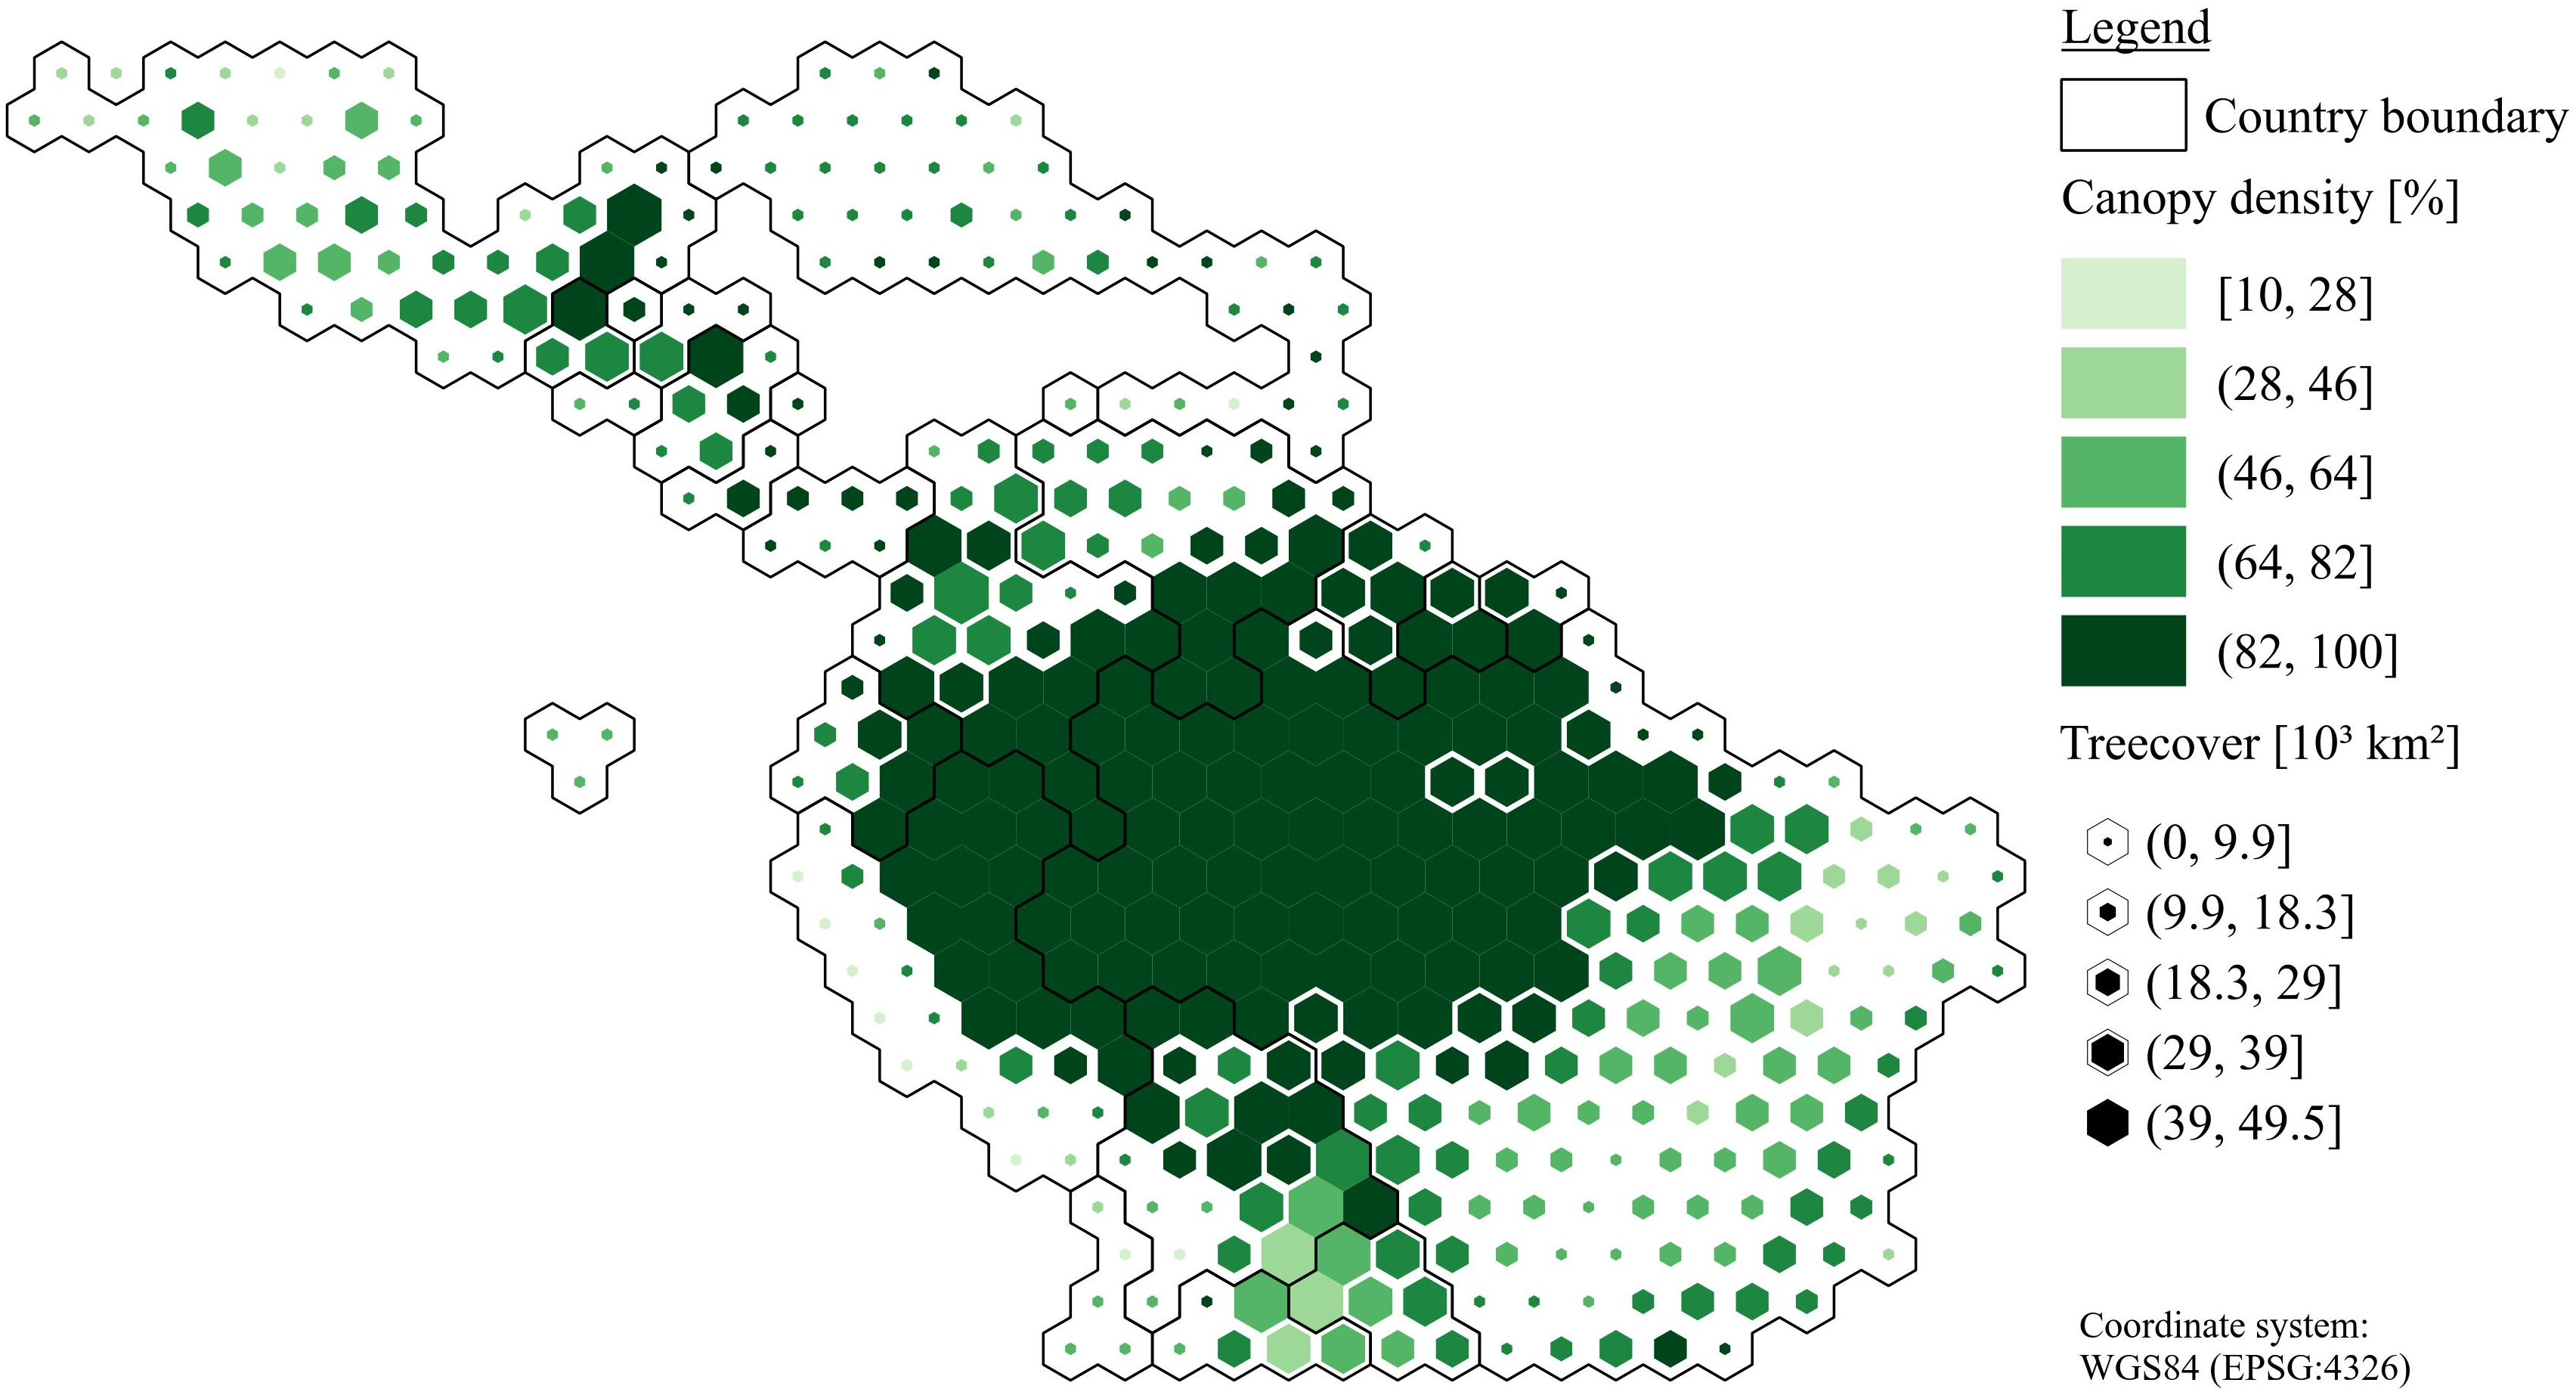
\includegraphics[scale=.86]{img/americas_treecover_frameless}
				\caption[Tree cover and canopy density in South America at 2000]{\textbf{Tree cover and canopy density in South America at 2000:} This map shows the tree cover and mean canopy density distribution at 2000. An unscaled hexagon covers an area of 0.5 decimal degrees which translates to approximately 49 thousand km$^2$ at the equator. Tropical rain forest in the center of the map is characterised by a tree cover between approximately 29 and 49 km$^2$ and canopy densities between 82 and 100 \%. The rain forest is surrounded by tropical moist forest with tree cover up to 49 km$^2$ but lower mean canopy densities between 10 and 82 \% as the rain forest. The tropical dry forest also known as Gran Chaco is located in the lower left of the map distributed over the countries Bolivia, Paraguay, and Argentina.}
				\label{fig:americas_tree_cover}
			\end{figure}
			\begin{figure}[ht]
				\centering
				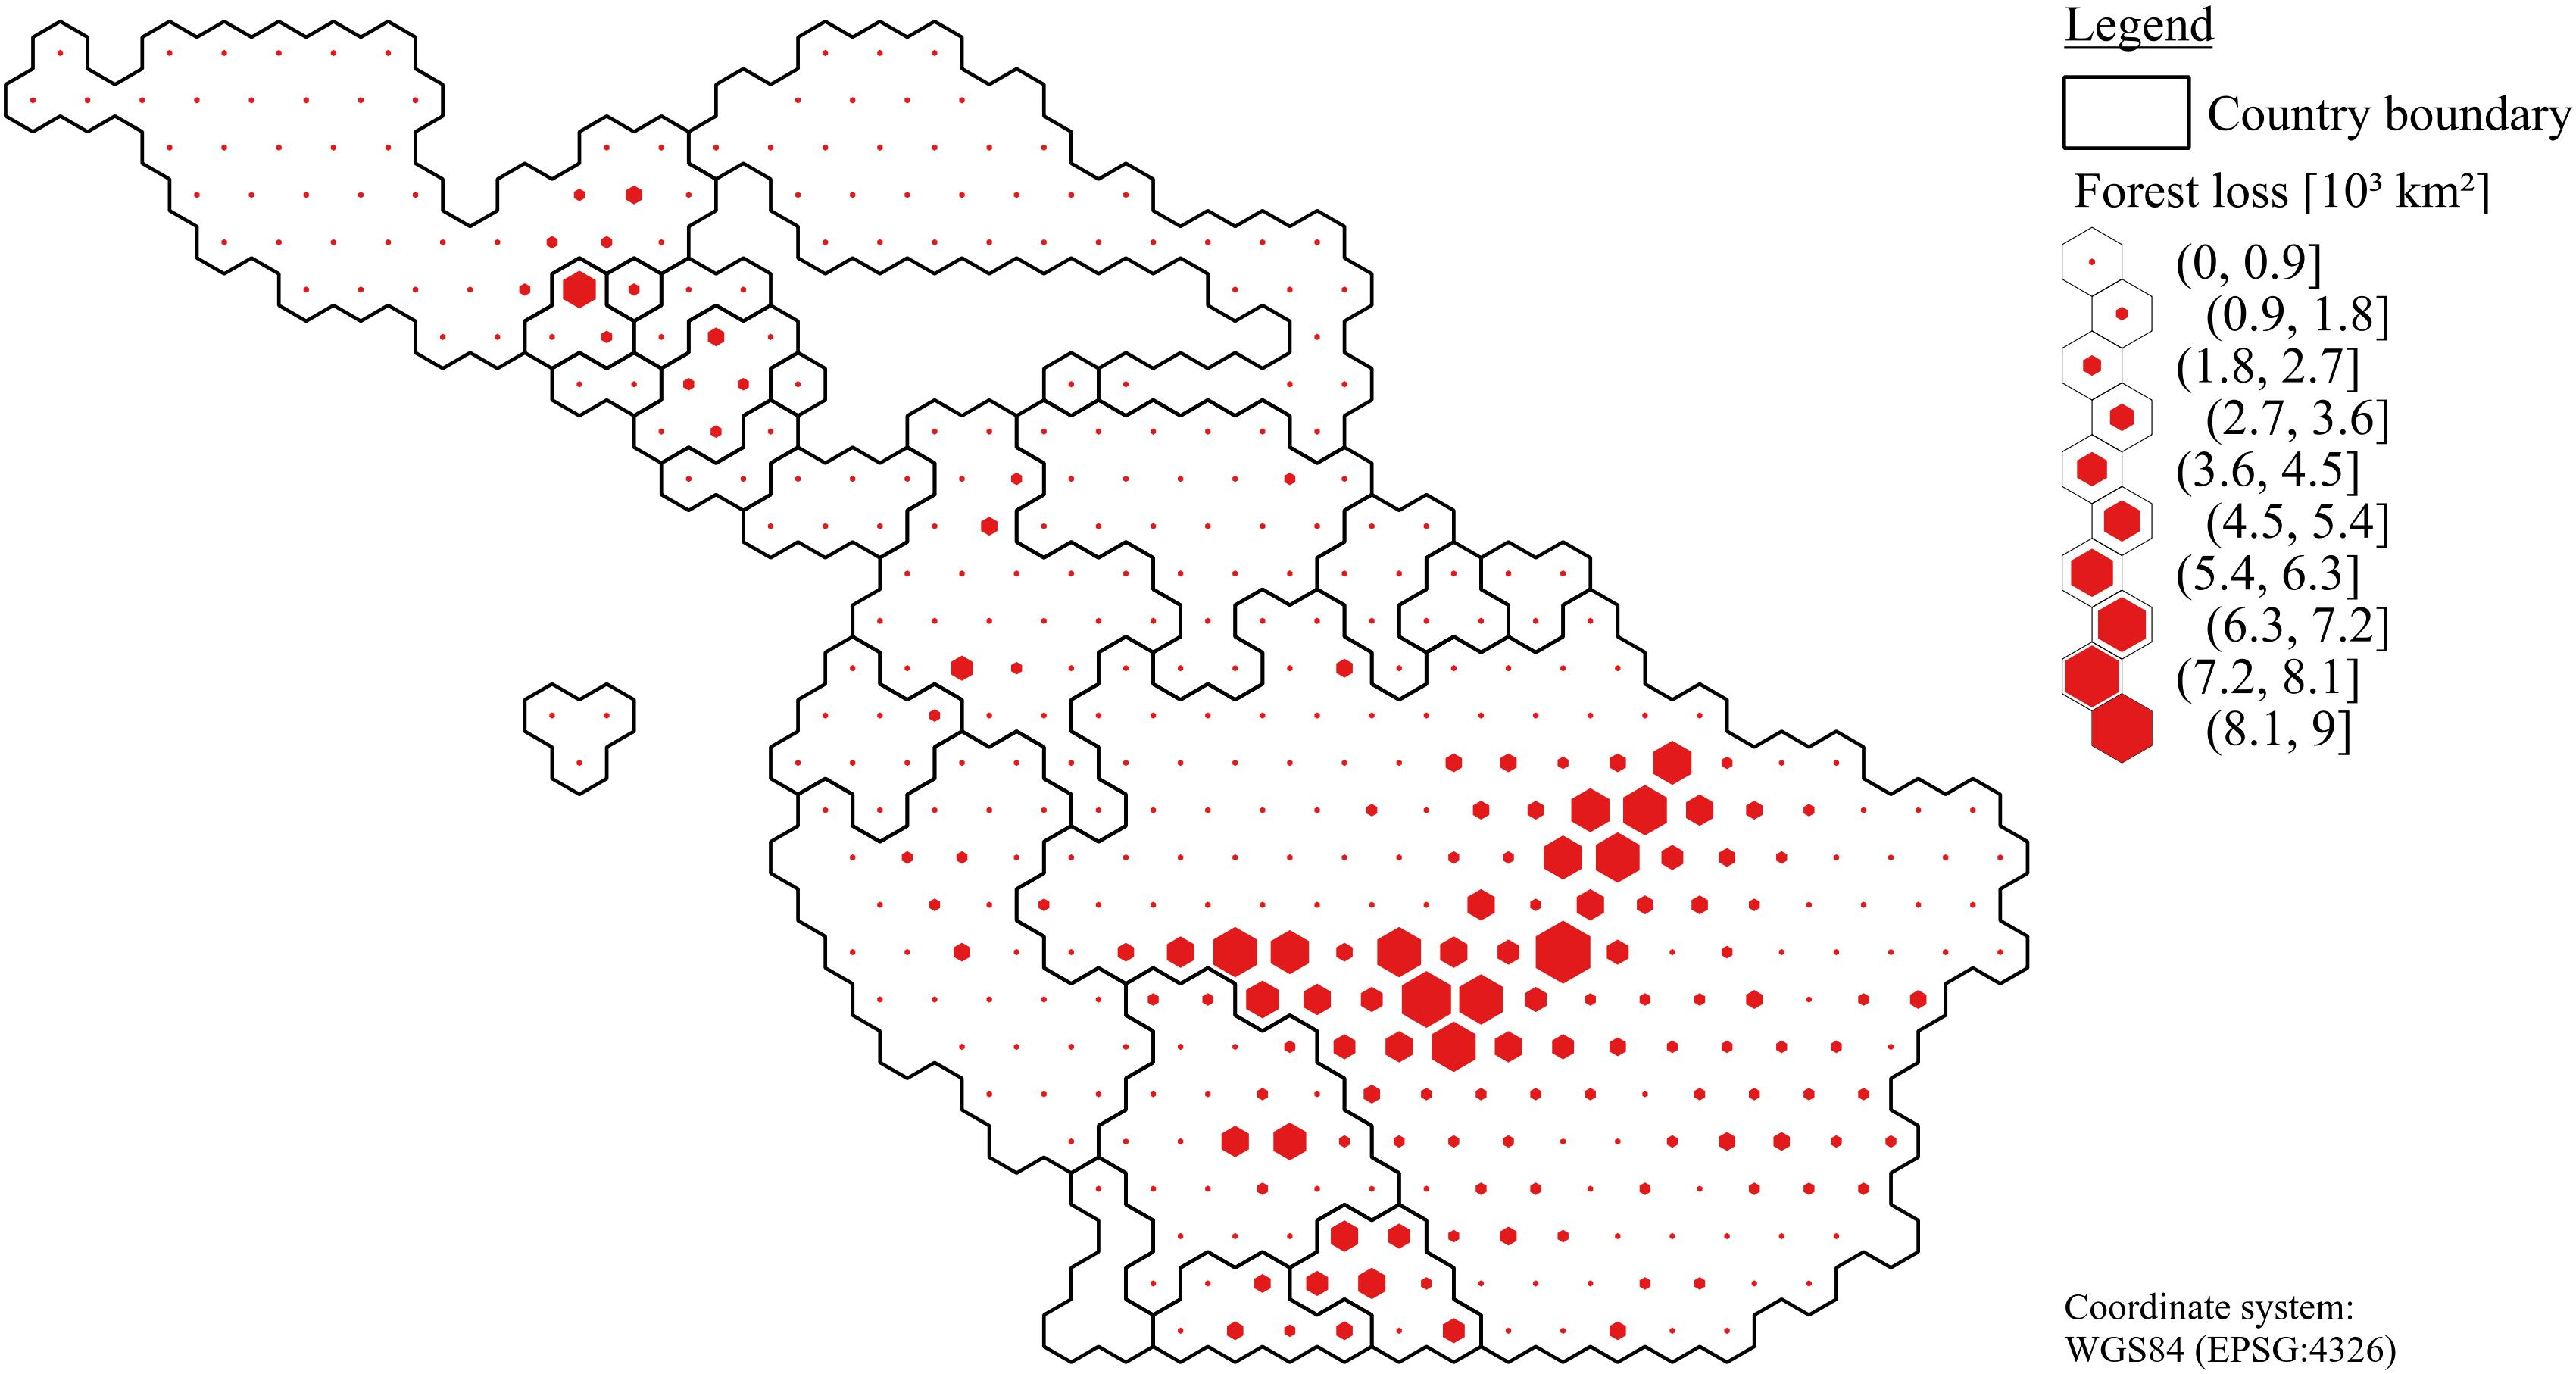
\includegraphics[scale=1]{img/americas_loss_frameless}
				\caption[Tree cover loss in South America between 2000 and 2010]{\textbf{Tree cover loss in South America between 2000 and 2010:} This map shows the tree cover loss within our study extent between 2000 and 2010. An unscaled hexagon covers an area of 0.5 decimal degrees which translates to approximately 49 thousand km$^2$ at the equator. Deforestation hot-spots with tree cover loss about approximately 2.7 thousand km$^2$ are located in Paraguay, Argentina, Bolivia, Brazil, Colombia, Peru, and Guatemala.}
				\label{fig:americas_loss}
			\end{figure}

			The map in figure \ref{fig:asia_tree_cover} shows the tree cover and canopy density distribution for Asia/Australia. In Asia the tropical rain forest is distributed over several southeast Asian islands like the Indonesian islands Sumatra, Borneo, Java, Papua etc., the Philippines, Malaysia, and Papua New Guinea. Generally the rain forest is characterised by high tree covers comparable to South America but in our map most of the islands are smaller than a single hexagon. Therefore, by our method to compute the hexagon scaling the size of the polygons don't reflect the tree cover as share of the landmass and most of them appear smaller. The mean canopy density of tropical rain forest is between 82 and 100 \% and the tree cover is above approximately 9.9 km$^2$. Tropical moist and dry forest are distributed over the continental Asia covering the countries India, Vietnam, Cambodia, Laos etc. These forests are characterised lower tree cover among 9.9 km$^2$ and canopy densities between 10 and 82 \% while the lower tree cover indicates that in southeast Asia deforestation occurs since the 1950s \citep{Kummer1994}. The map in figure \ref{fig:asia_loss} shows the distribution of tree cover loss in Asia/Australia for the time period 2000 till 2010. During this period an area of approximately 196 thousand km$^2$ is exposed to deforestation as table \ref{tab:proximate_driver} in the appendix suggests. For this region we identified the following countries as deforestation hot-spots with deforestation areas per hexagon of approximately 2.7 to 9 thousand km$^2$: Indonesia, continental and insular Malaysia, Vietnam, Cambodia, and Laos.
			\begin{figure}[ht]
				\centering
				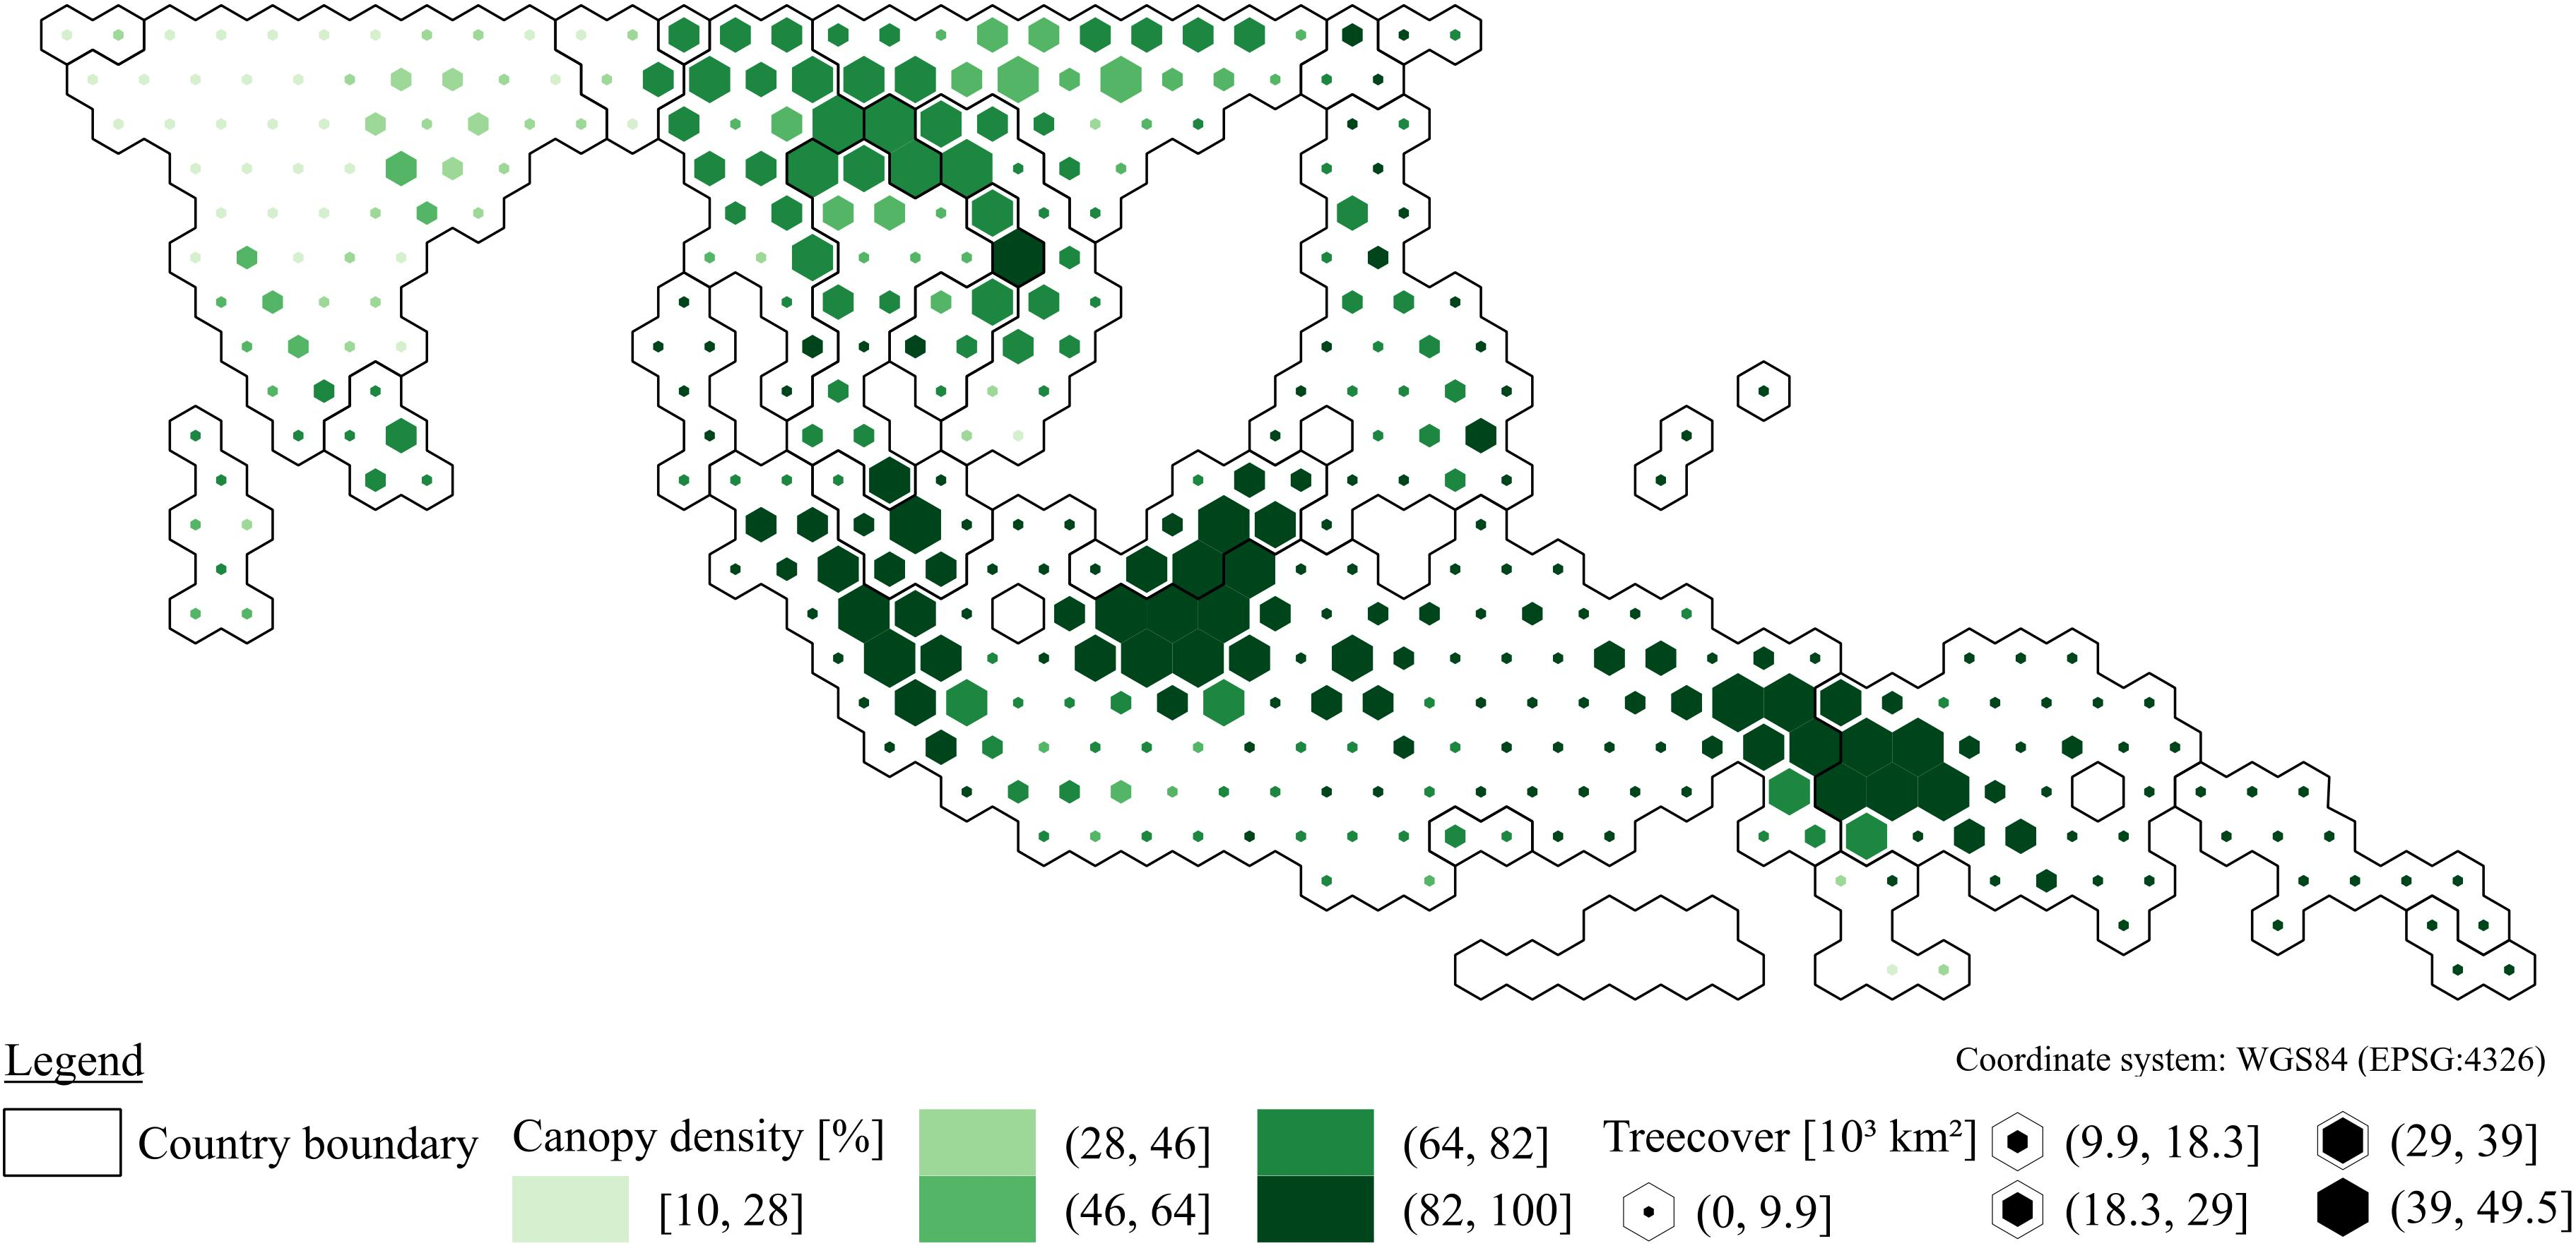
\includegraphics[scale=1]{img/asia_treecover_frameless}
				\caption[Tree cover and canopy density in Asia/Australia at 2000]{\textbf{Tree cover and canopy density in Asia/Australia at 2000:} This maps shows the tree cover and mean canopy density distribution within our study extent at 2000. An unscaled hexagon covers an area of 0.5 decimal degrees which translates to approximately 49 thousand km$^2$ at the equator.}
				\label{fig:asia_tree_cover}
			\end{figure}
			\begin{figure}[ht]
				\centering
				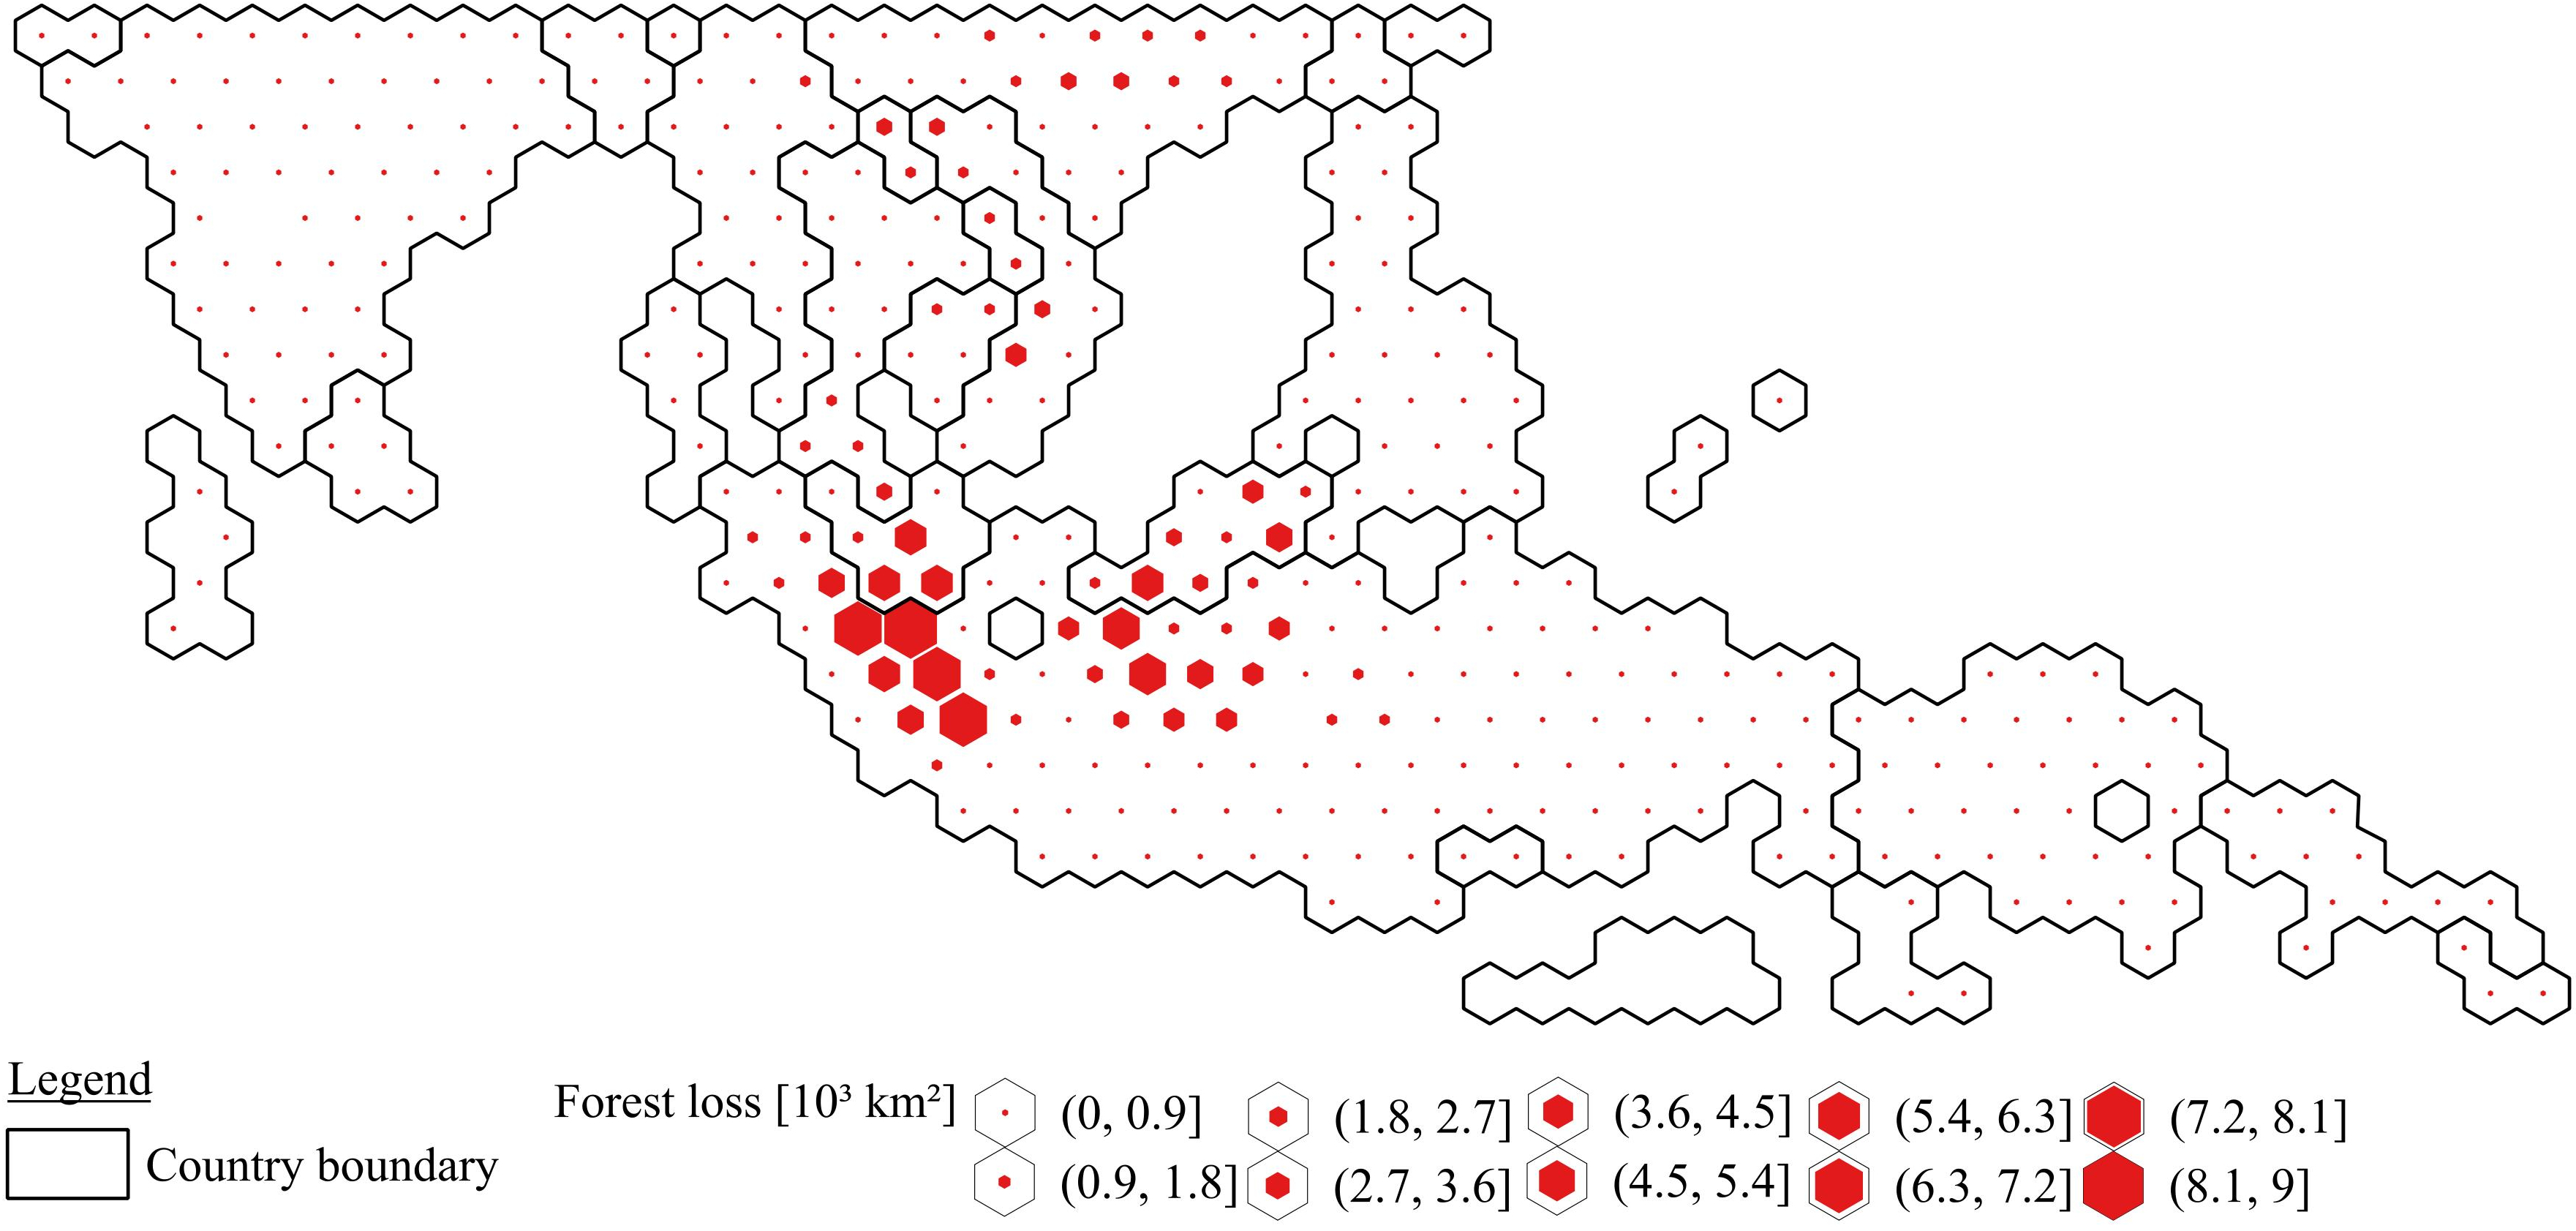
\includegraphics[scale=1]{img/asia_loss_frameless}
				\caption[Tree cover loss in Asia/Australia between 2000 and 2010]{\textbf{Tree cover loss in Asia/Australia between 2000 and 2010:} This map shows the tree cover loss within our study extent between 2000 and 2010. An unscaled hexagon covers an area of 0.5 decimal degrees which translates to approximately 49 thousand km$^2$ at the equator.}
				\label{fig:asia_loss}
			\end{figure}

			Figure \ref{fig:africa_tree_cover} shows the tree cover and canopy density distribution over Africa. In Africa the tropical rain forest is distributed over the following central African countries: Democratic Republic of the Congo, Republic of the Congo, Equatorial Guinea, Gabon, Cameroon, and partial in Ghana, Ivory Coast, and Liberia. In our map this type of forest is characterised by a dense tree cover between 39 and 49 thousand km$^2$ per hexagon while the canopy density between 64 and 100 \% does not separate it from the moist type as good as in South America and Asia/Australia. The rain forest is surrounded by tropical moist forest with a dense tree cover between 18 and 49 thousand km$^2$ while the mean canopy density between 10 and 82 \% is sparser then tropical rain forest. Countries covered by the moist forest type are the following examples: Angola, Uganda, Central African Republic, Zambia, Madagascar etc. Tropical dry forest is characterised by a sparse tree cover among approximately 18 thousand km$^2$ and canopy densities between 10 and 46 \%. Mozambique, Tanzania, and Nigeria are examples for countries covered partial by tropical dry forest. The map in figure \ref{fig:africa_loss} shows the regions which are exposed to tree cover loss in Africa for the time period 2000 till 2010. During the first decade of 2000 an area of approximately 174 km$^2$ was deforested as table \ref{tab:proximate_driver} in the appendix suggests. With tree cover loss between 4.5 and 9 thousand km$^2$ we identified the following countries as deforestation hot-spots: Ivory Coast, Democratic Republic of the Congo, Angola, Zambia, Mozambique, Madagascar, and Tanzania. 
			\begin{figure}[ht]
				\centering
				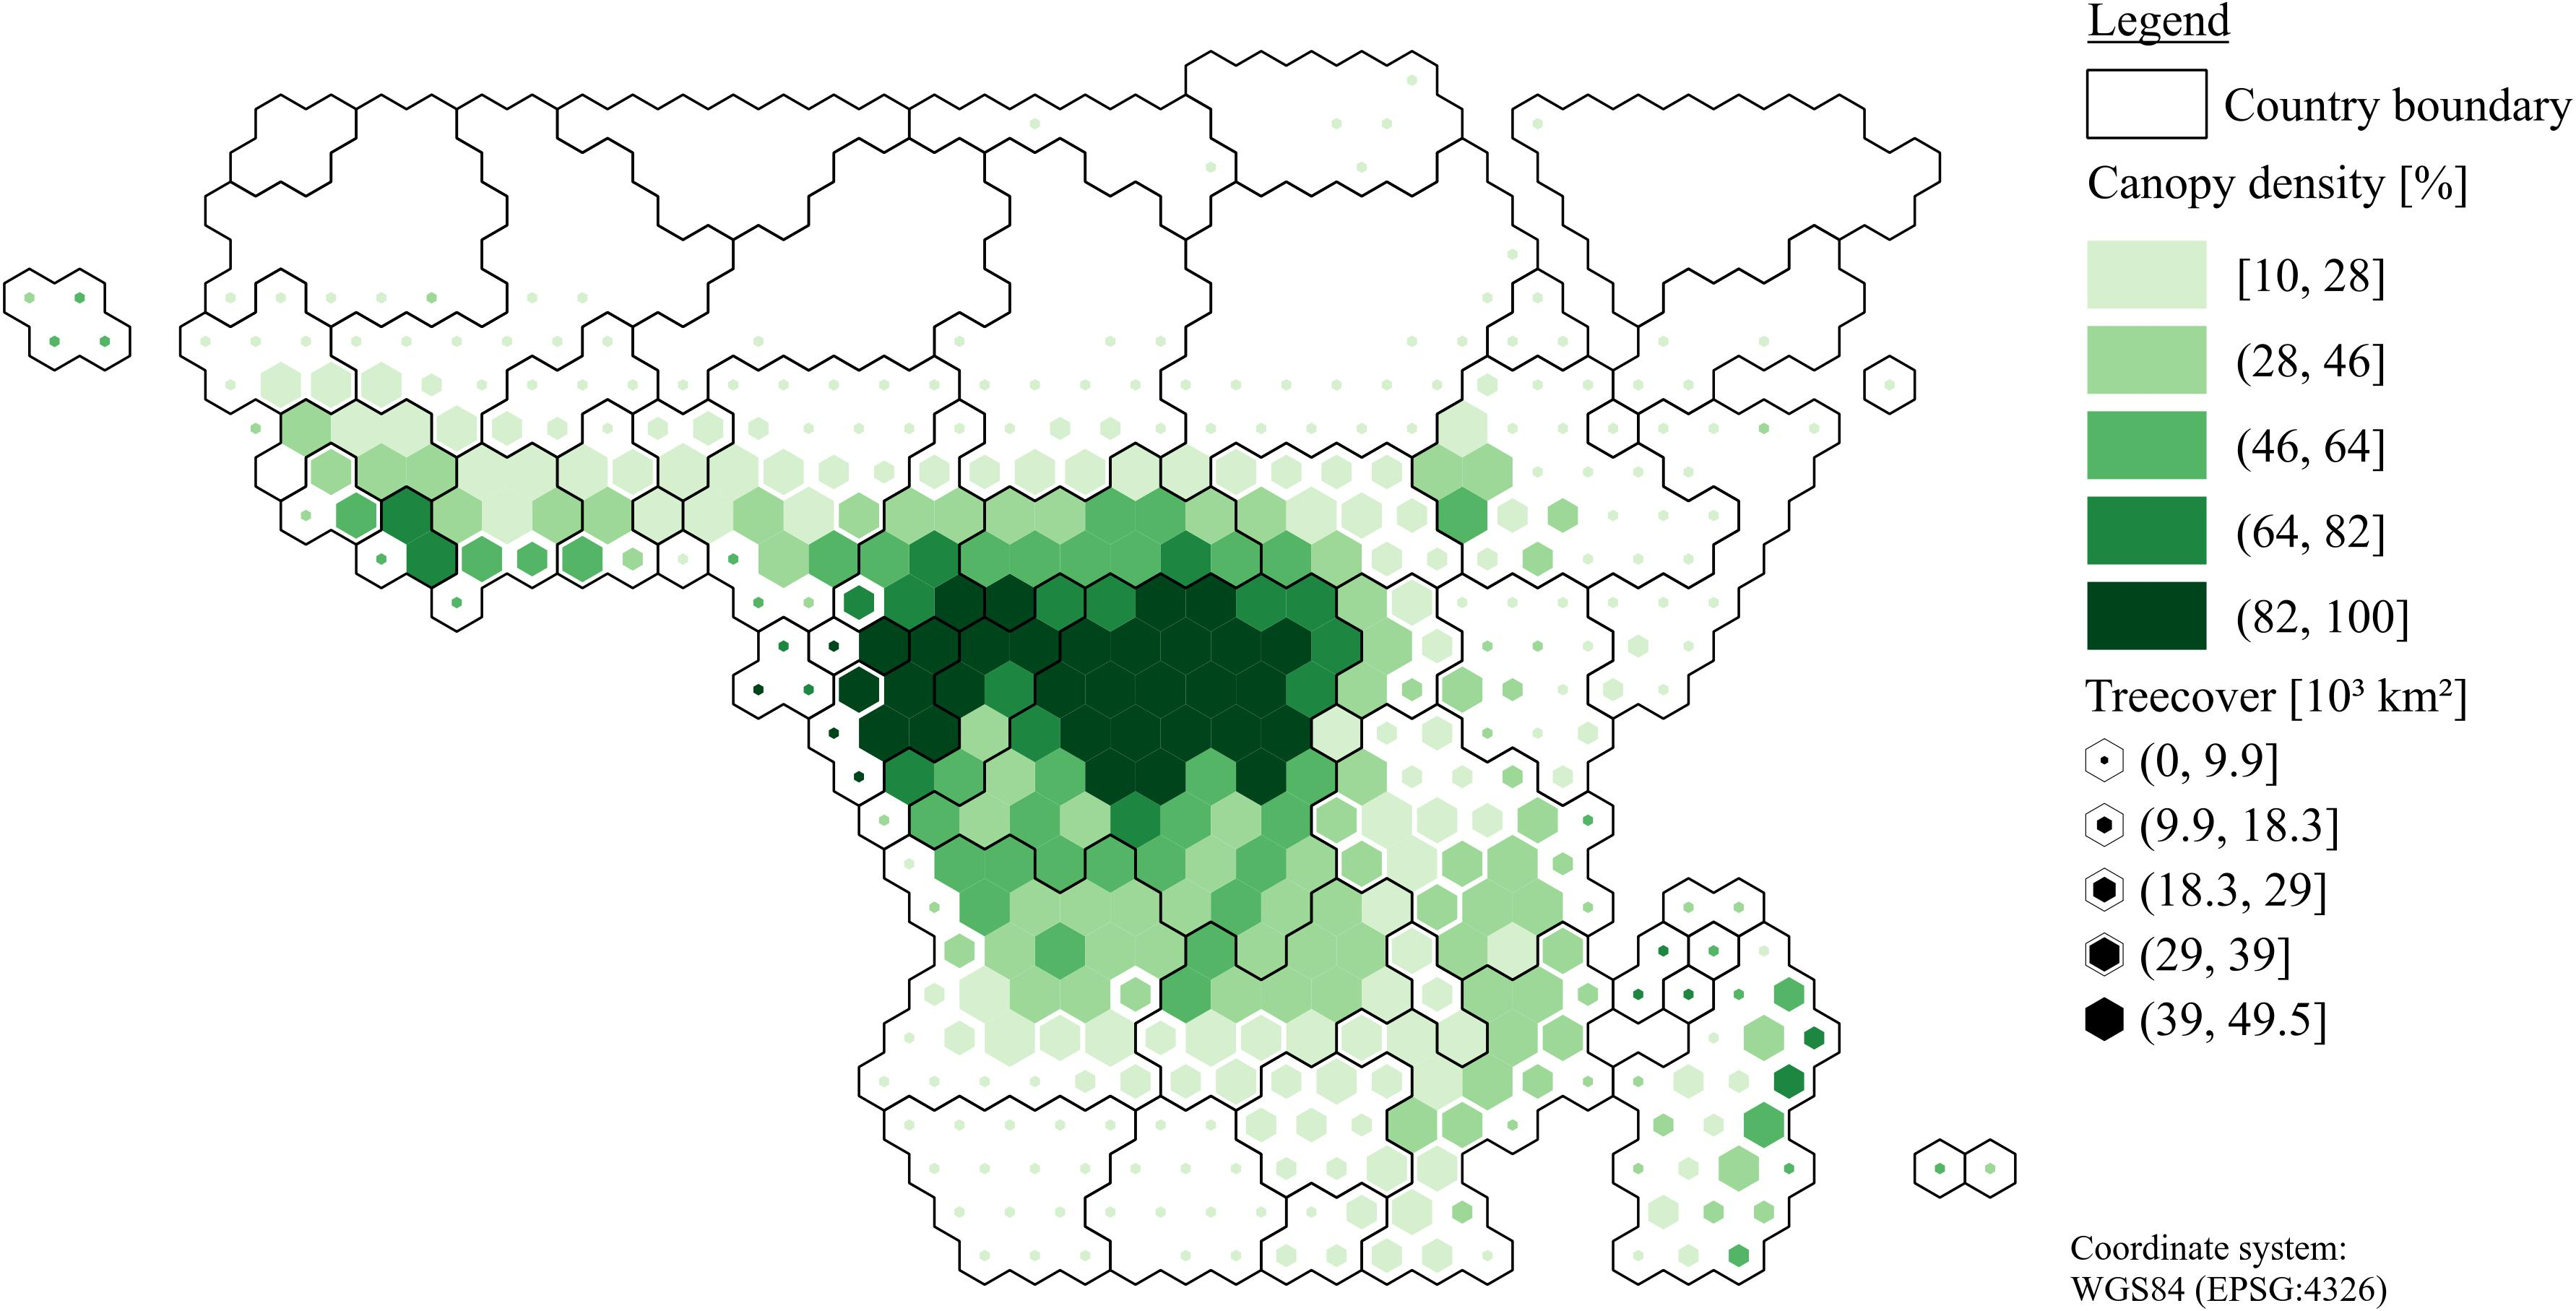
\includegraphics[scale=1]{img/africa_treecover_frameless}
				\caption[Tree cover and canopy density in Africa at 2000]{\textbf{Tree cover and canopy density in Africa at 2000:} This maps shows the tree cover and mean canopy density distribution within our study extent at 2000. An unscaled hexagon covers an area of 0.5 decimal degrees which translates to approximately 49 thousand km$^2$ at the equator.}
				\label{fig:africa_tree_cover}
			\end{figure}
			\begin{figure}[ht]
				\centering
				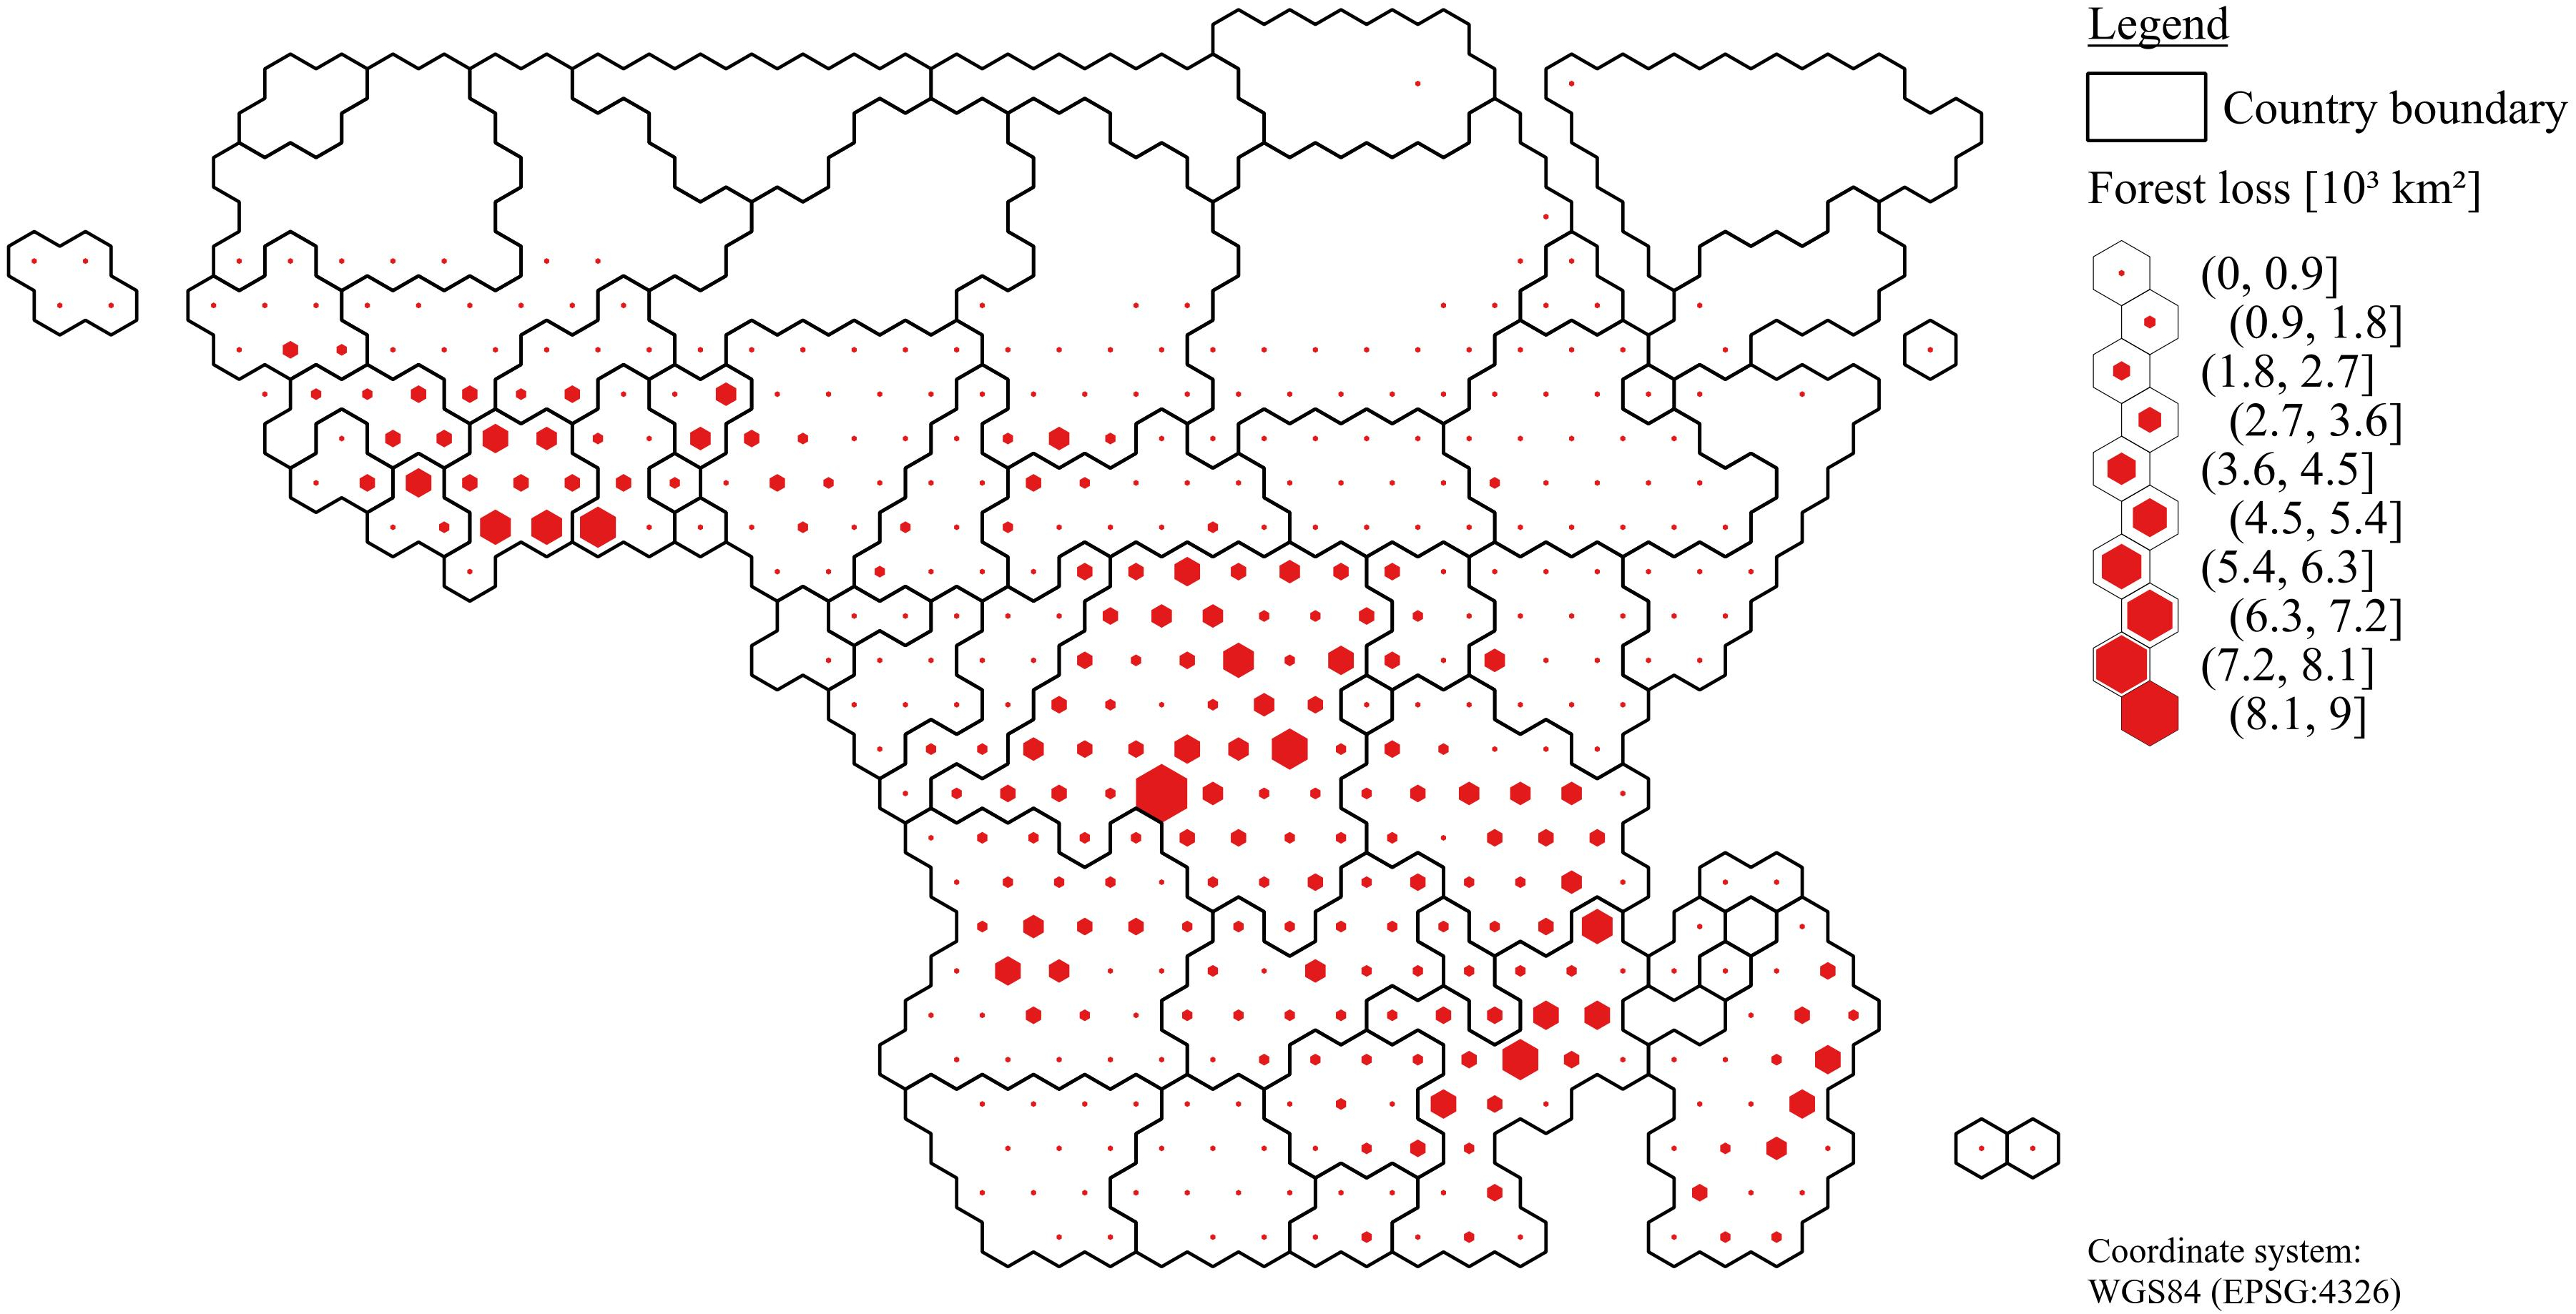
\includegraphics[scale=1]{img/africa_loss_frameless}
				\caption[Tree cover loss in Africa between 2000 and 2010]{\textbf{Tree cover loss in Africa between 2000 and 2010:} This map shows the tree cover loss within our study extent between 2000 and 2010. An unscaled hexagon covers an area of 0.5 decimal degrees which translates to approximately 49 thousand km$^2$ at the equator.}
				\label{fig:africa_loss}
			\end{figure}

		\subsection{Proximate deforestation driver}
		\label{subsec:results_proxy_deforestation_driver}
			\note{Goal (review):} Goal is to estimate the distribution of proximate deforestation drivers on global, continental, and regional scale for the tropics between 2001 and 2010. We used a approach by superimposing the gfc annual loss and the gl30 land cover map from 2010. We carefully selected the target canopy density by analyzing the tree cover agreement between both layers at 2000. We filtered the gfc data by applying the canopy density interval within $(10,100]$. By filtering is meant that we used only annual loss which occur in this interval. Also we selected only gain data from gfc which is connected to a previous loss. We applied a reclassification after superimposing both layers to handle the great share of pixels classified as forest. We used clustering to aggregate these pixels and applied a square sized buffer of 500 meter. We determined the most frequent class within this buffer and assigned it to the cluster.
            
            \note{South America:}
			\begin{figure}[ht]
				\centering
				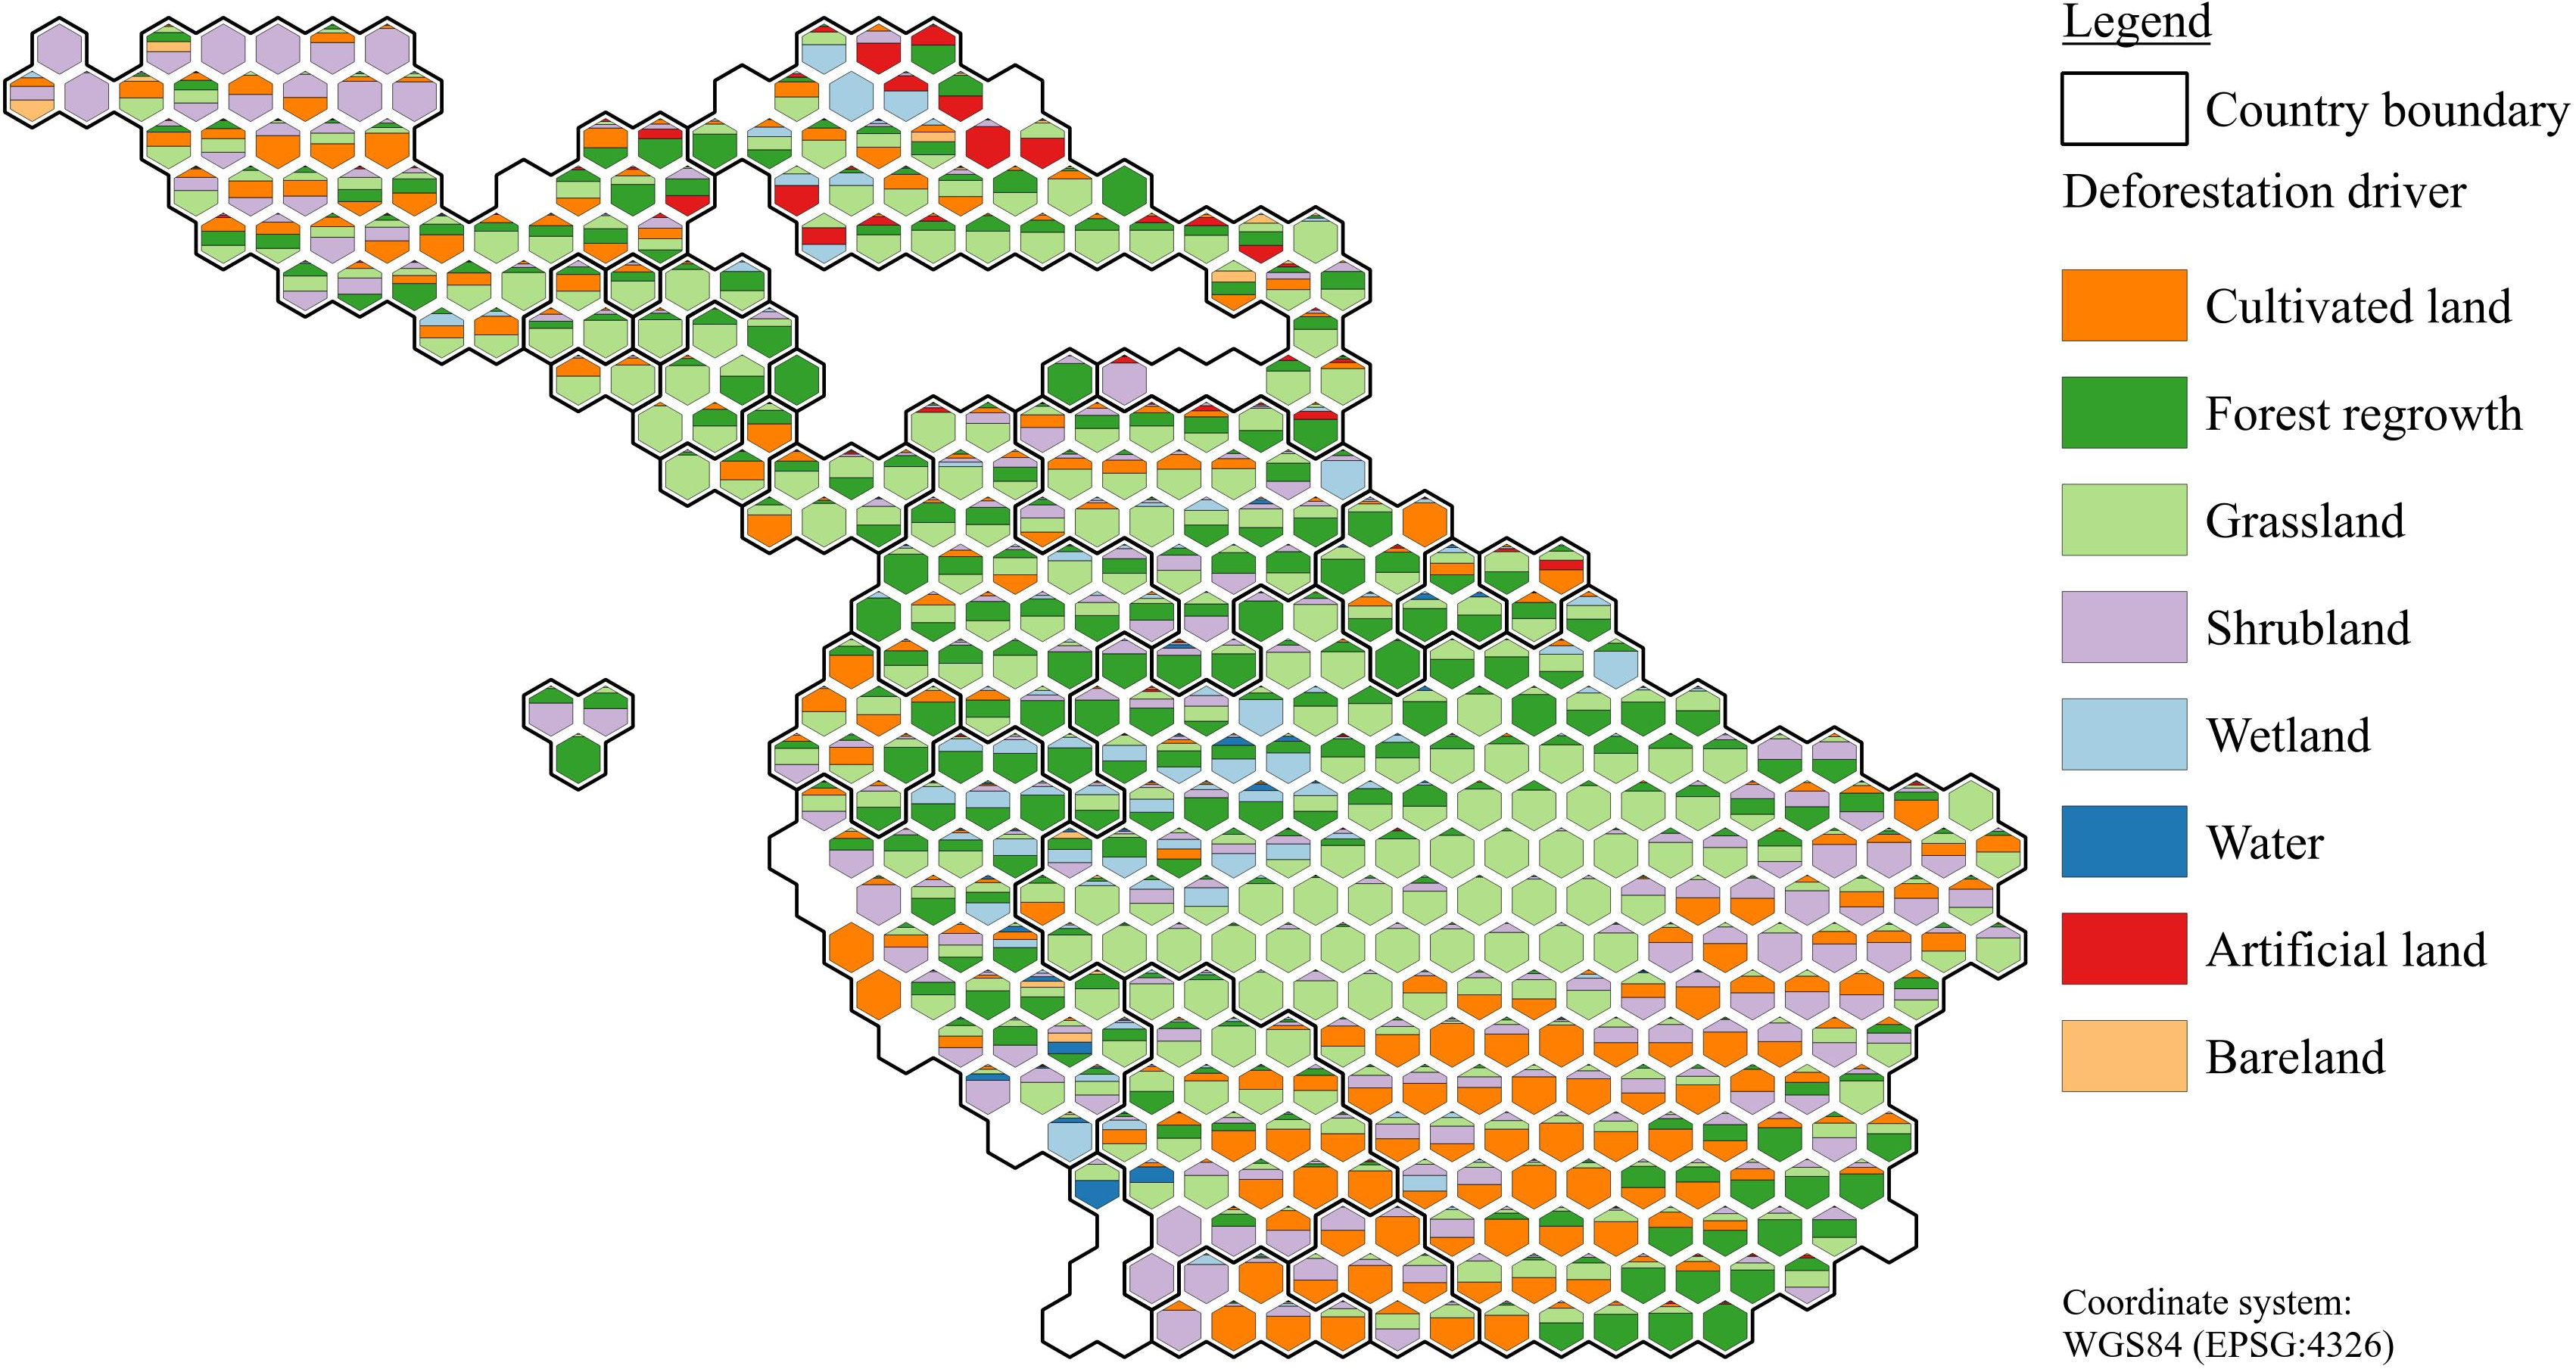
\includegraphics[scale=1]{img/americas_driver_frameless}
				\caption[Map of proximate deforestation driver in South America]{}
				\label{fig:americas_driver}
			\end{figure}

            \note{Asia/Australia:}
			\begin{figure}[ht]
				\centering
				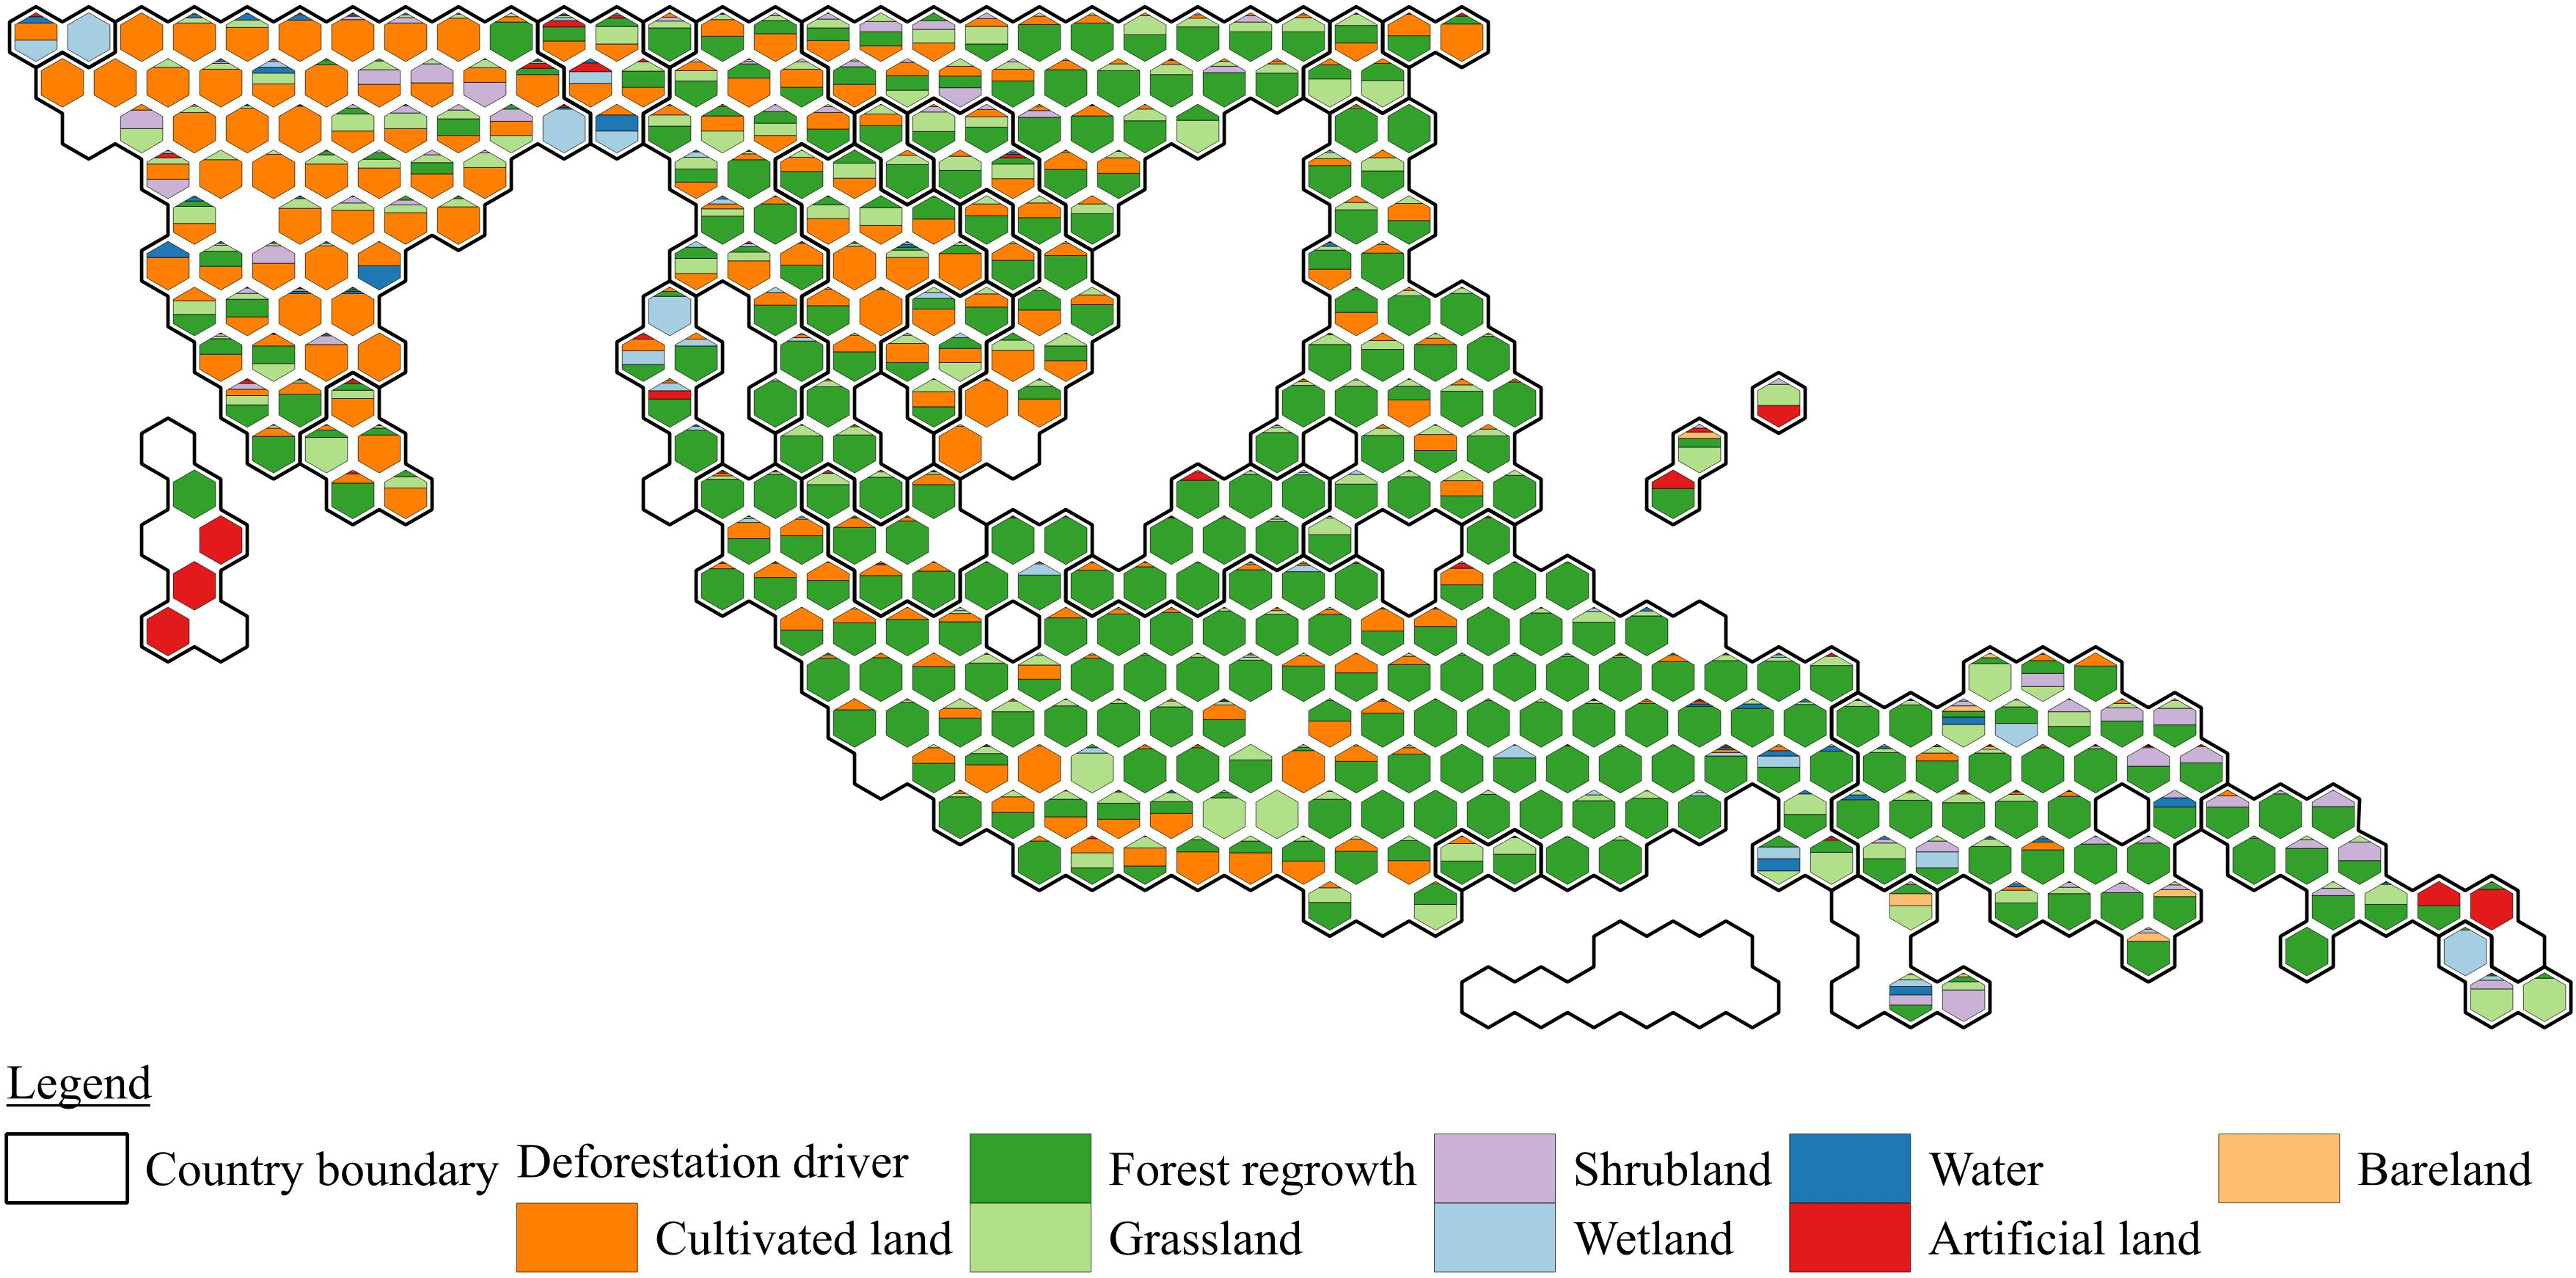
\includegraphics[scale=1]{img/asia_driver_frameless}
				\caption[Map of proximate deforestation driver in Asia/Australia]{}
				\label{fig:asia_driver}
			\end{figure}

            \note{Africa:}
			\begin{figure}[ht]
				\centering
				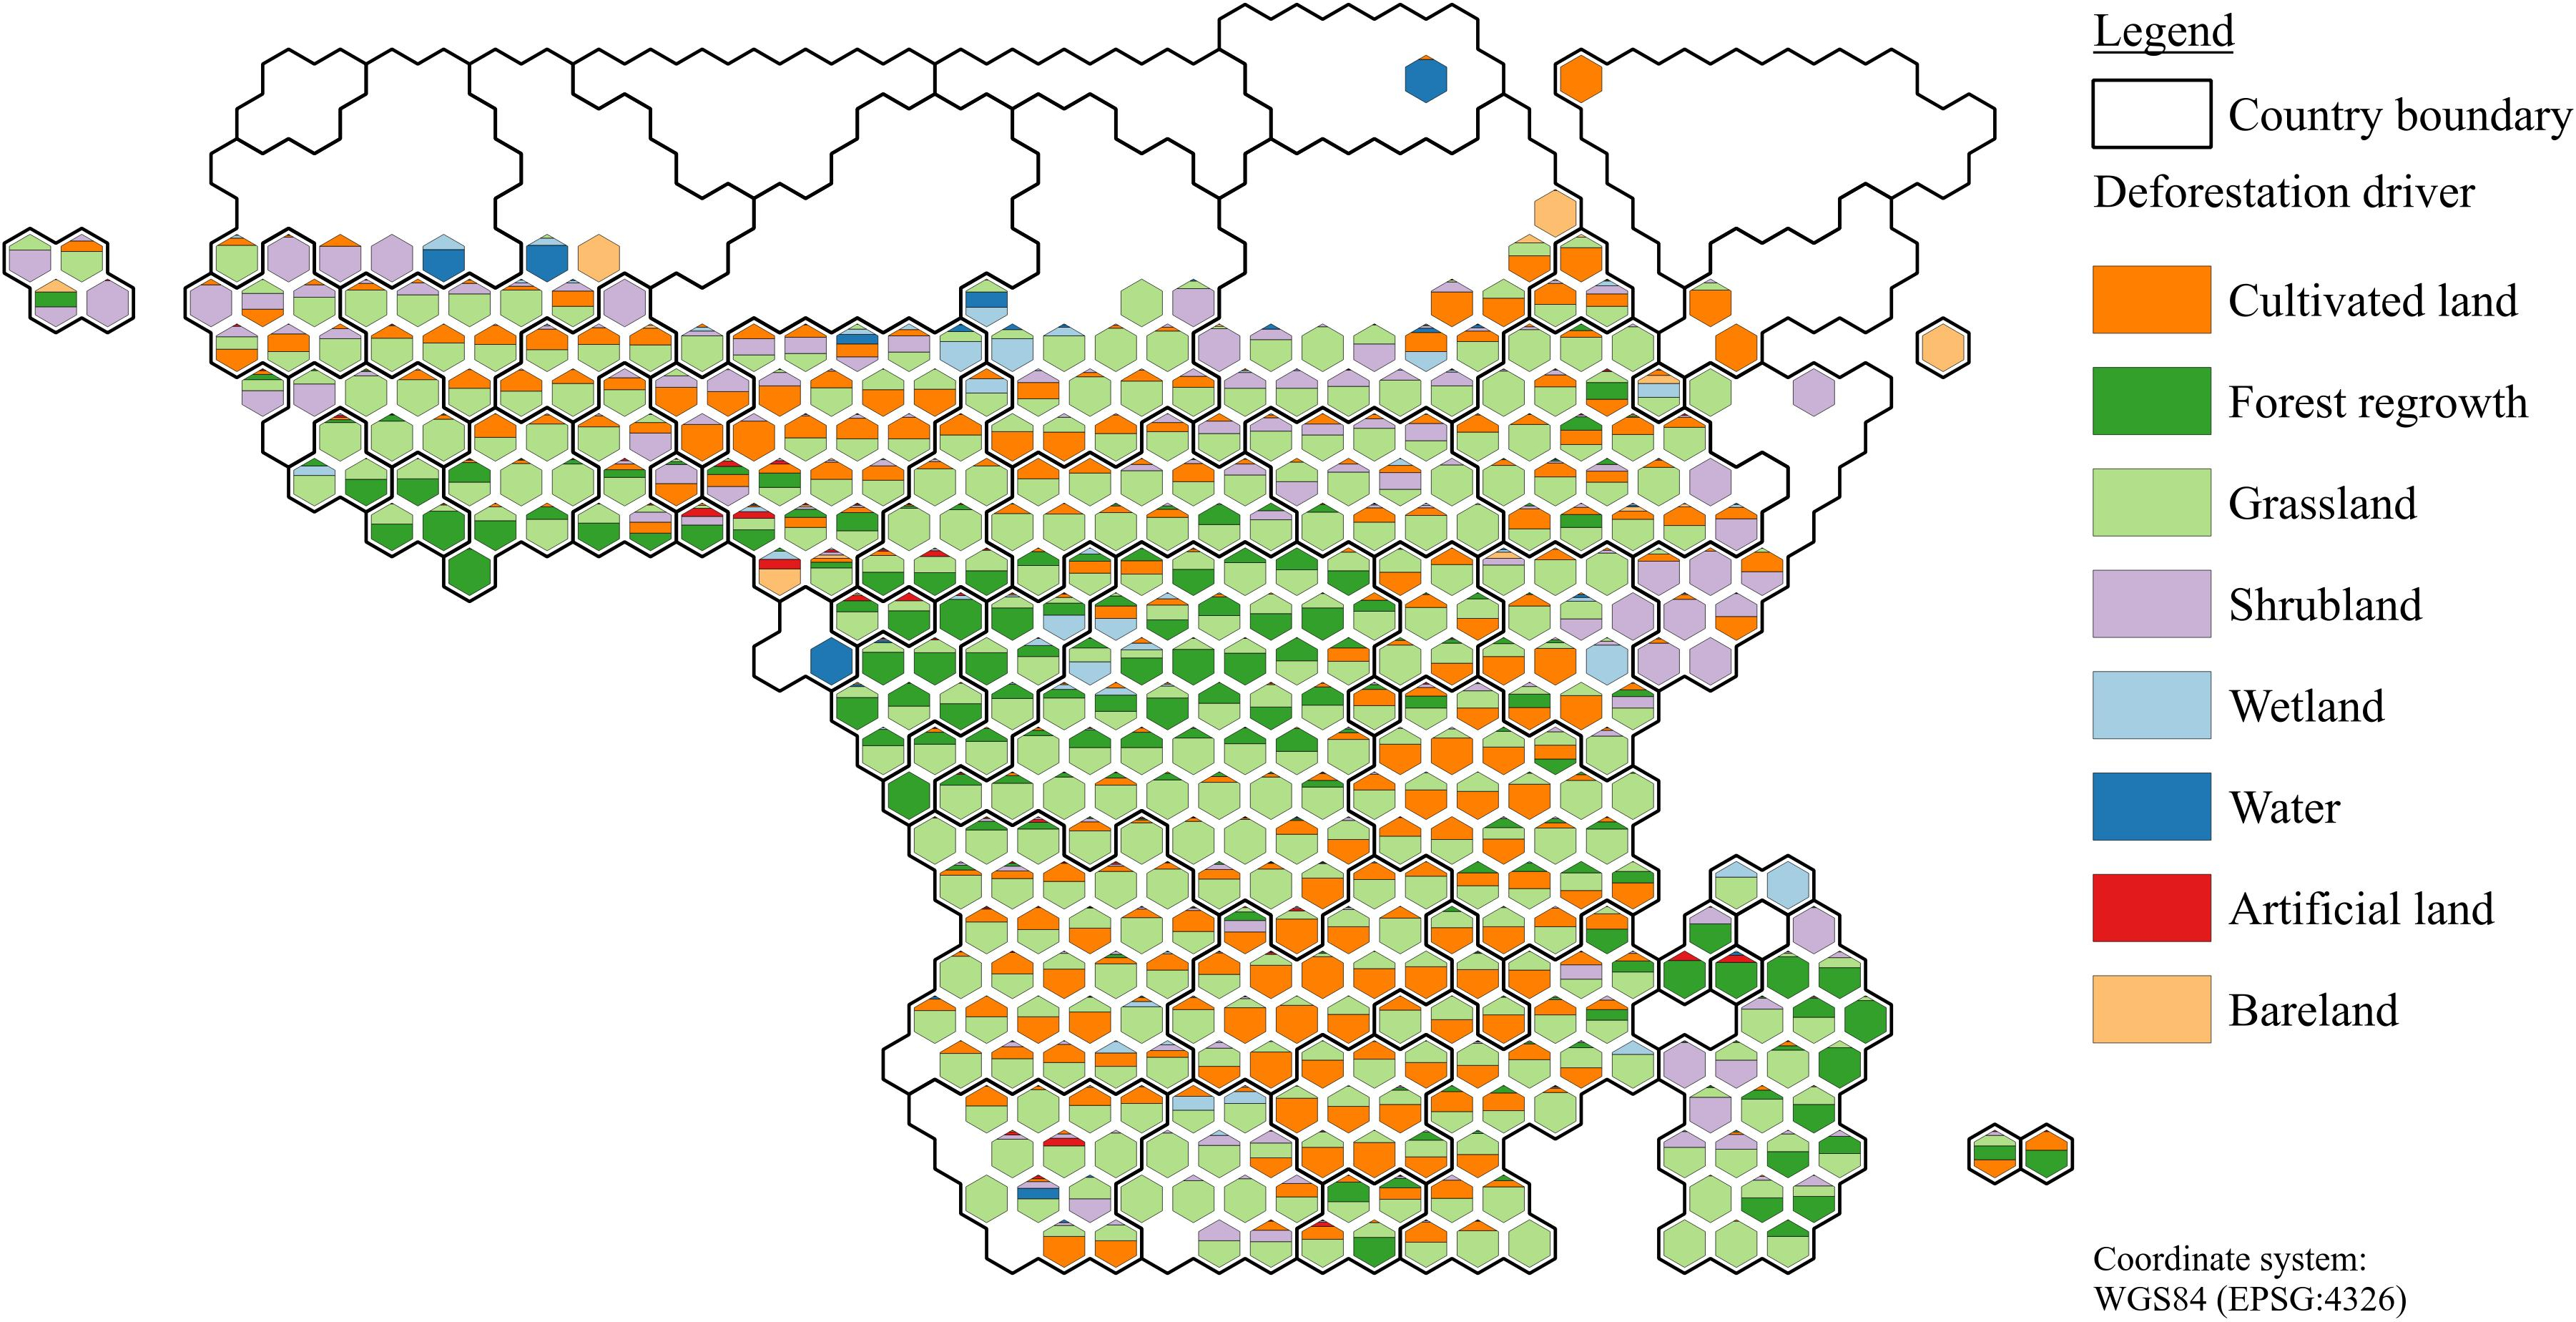
\includegraphics[scale=1]{img/africa_driver_frameless}
				\caption[Map of proximate deforestion driver in Africa]{}
				\label{fig:africa_driver}
			\end{figure}

		\subsection{Accuracy assessment}
		\label{subsec:results_accuracy_assessment}
		%TODO distribution is it in line with global estimates
			\note{Goal (review):} Goal is the assessment of the accuracy of our proximate deforestation driver predictions. We created a set of ground truth data by sampling our proximate deforestation driver layers. In each continental region we select per random 10 tiles and draw 200 samples per tile. The 200 samples comprises pixels over the full value range of our proximate deforestation driver classes. We imported the prepared sample to our JavaScript application and subsequently classified each sample with a label by visual interpretation of google earth imagery. To determine the accuracy we used a confusion matrix and the derived metrics.

			\note{Results (review):} Table \ref{tab:results_confusion_matrix} shows the confusion matrix to determine the accuracy of our predictions where the term reference refers to the labeling of pixel by our visual interpretation and predictions refer to the labeling of our proximate driver predictions. The abbreviations PAc, UAc, OvAc, Com, Om, Tot, and Kappa refer to the terms Producers-Accuracy, Users-Accuracy, Overall-Accuracy, Error of Commission, Error of Omission, row or column total, and Kappa Coefficient. From the 6000 samples we draw from our study extent 14 \%, 20 \%, 22 \%, 32 \%, 8 \%, 2 \%, 0.5 \%, 2 \%, and 0.5 \% account for cultivated land (10), tree cover (20), regrowth (25), shrubland (40), wetland (50), water (60), artificial land (80), and bareland (90), respectively. Our method predicts a distribution of 15 \%, 18 \%, 27 \%, 31 \%, 7 \%, 1 \%, 0.8 \%, 1 \%, and 0.2 \% for the land cover classes 10, 20, 25, 30, 40, 50, 60, 80, and 90, respectively.
			Highest producers accuracy is achieved the regrowth class with 88 percent. The prediction of this class was achieved by including global forest change gain data within our target canopy density. During building our reference data set per visual interpretation we determined this class by following these rules. We checked the surroundings and the corresponding pixel for signs of road networks and infrastructure. Further we checked if the canopy shows signs of age class forest and line patterns which show the establishment of artificial introduced forest cover. During the visual interpretation we recognized that a large portion of the regrowth class is occupied by plantations especially in Americas and Asia. For Asia a major share was occupied by palm oil or other plantations. It must be mentioned that here the deforestation within our temporal frame is not coercively the clearing of natural cover/primary forest it shows it shows also rotational cycles of deforestation reforestation.
			The second highest accuracy with 85 (producers accuracy) was achieved in the prediction of cultivated land where only 15 percent could be identified as error of commission. 8.2 percent are classified as forest or regrowth which could reveal zones of shifting agriculture or temporal issues. To identify this class during our visual interpretation we applied nearly the same rules as the detection of regrowth checking for infrastructure but here no canopy should be identified. Further we checked for large scale square patterns which is shown by large scale commodity driven agriculture. Especially the small scale agriculture was hard detect because these class of agriculture often show no regular patterns of forest clearing and are often accompanied by selective logging. Further it should be mentioned common practice of small scale agriculture is inhomogeneous over the regions Americas, Asia and Africa. Another good indicator for cultivated land is the appearance of tillage patterns on high resolution imagery. Cultivated land comprises a large variety of different use cases. 
			Grassland shows an accuracy of 77 at an error of commission of 23 percent. The error could lead back to classification errors by GlobeLand30 or land cover change dynamics and the temporal time frame. For visual interpretation cultivated land and grassland share some common properties like square shaped clearings and infrastructure in the surroundings. But grassland is also defined by the occurrence of shrubs and single trees within its extent. To really determine the differences between both classes high resolution imagery is required. In Americas the grassland patches could often be identified as used for cattle ranching. During visual interpretation we recognized frequently the occurrence of water holes. Africa showed the occurrence of natural grasslands and Asia bla.
			\begin{table}[ht]
				\centering
				\caption[Confussion matrix]{\textbf{Confussion matrix for accuracy assessment:} We draw 6000 samples from 10 random selected tiles from the three regions Americas, Asia and Africa. Labels refer to our proximate deforestation driver classes which correspond to GlobeLand30 classification schema in table \ref{tab:gl30_classes}. Reference refers to the samples we classified by visual interpretation of external imagery and predictions refer to the label the sample has in our proximate driver product. The abbreviations PAc, UAc, OvAc, Com, Om, Tot, and Kappa refer to the terms Producers-Accuracy, Users-Accuracy, Overall-Accuracy, Error of Commission, Error of Omission, row or column total, and Kappa Coefficient.}
				\label{tab:results_confusion_matrix}
				\begin{tabular}{llrrrrrrrrrrrr}
					\hline
					& & \multicolumn{9}{c}{Reference} & & & \\\cline{3-11}
					& Cls & 10 & 20 & 25 & 30 & 40 & 50 & 60 & 80 & 90 & Tot & UAc & Om \\\hline
					\multirow{9}{*}{\STAB{\rotatebox[origin=c]{90}{Prediction}}}
					& 10 & 730 & 37 & 62 & 15 & 16 & 2 & 3 & 5 & 0 & 870 & .84 & .16 \\ 
					& 20 & 41 & 744 & 56 & 189 & 31 & 12 & 0 & 15 & 4 & 1092 & .68 & .32 \\ 
					& 25 & 29 & 202 & 1155 & 172 & 22 & 10 & 5 & 11 & 4 & 1610 & .72 & .28 \\ 
					& 30 & 36 & 187 & 32 & 1466 & 73 & 21 & 0 & 17 & 0 & 1832 & .80 & .20 \\ 
					& 40 & 14 & 21 & 4 & 41 & 352 & 1 & 1 & 2 & 1 & 437 & .81 & .19 \\ 
					& 50 & 0 & 5 & 3 & 10 & 4 & 50 & 0 & 1 & 0 & 73 & .68 & .32 \\ 
					& 60 & 2 & 1 & 0 & 3 & 0 & 2 & 18 & 2 & 0 & 28 & .64 & .36 \\ 
					& 80 & 3 & 3 & 0 & 1 & 1 & 1 & 0 & 40 & 0 & 49 & .82 & .18 \\ 
					& 90 & 0 & 0 & 0 & 1 & 0 & 0 & 0 & 3 & 5 & 9 & .56 & .44 \\\hline 
					& Tot & 855 & 1200 & 1312 & 1898 & 499 & 99 & 27 & 96 & 14 & 6000 & & \\
					& PAc & .85 & .62 & .88 & .77 & .71 & .51 & .67 & .42 & .36 & Kappa & \multicolumn{2}{r}{OvAc} \\
					& Com & .15 & .38 & .12 & .23 & .29 & .49 & .33 & .58 & .64 & .69 & \multicolumn{2}{r}{.76} \\ \hline
				\end{tabular}
			\end{table}

	\section{Emissions}
		\note{Goal (review):} Our goal is to estimate the emissions emitted by proximate deforestation driver. We estimated the emissions from the removal of aboveground biomass and through the change of soil organic carbon content. Detailed below are the pdd classes we assumed as deforestation to estimate the agb emissions: 10, 25, 30, 40, 80, 90. To approximate the emissions by soil organic carbon change we used the transition pathways from don et al. We estimated soc for two different scenarios with the following conditions: scenario one (SC1) all transitions occur in primary forest and scenario two (SC2) by using the intact forest landscape layer we distinguished between primary forest and secondary forest. The first scenario can be seen as liberal estimate and the second scenario as conservative estimate. We aggregated our results on global and continental scale. 

	\section{Ecosystem service values}
		Our goal is to estimate the monetary loss of \ac{ESV} by the aggregated \ac{PDD} at a global and continental scale between 2001 and 2010. Whereas a study targeting regional scale aggregation could easily performed with our data. Additionally, we approximated the monetary gain if the former tree cover is converted to a certain type of \ac{LC}. We refer to this gain as \ac{ESV} gain. Further, we compute the balance between \ac{ESV} loss and gain to estimate the net change of \ac{ESV} in the tropical zone. We applied three datasets which estimate the monetary value of ecosystems on a global scale namely the following data: \citet{Groot2012}, \citet{Costanza2014}, and \citet{Siikamaki2015}. We refer to this datasets as Co, Dg, and Wb. To compute the monetary loss of \ac{ESV} we selected the following \ac{PDD} classes as anthropogenic deforestation: cultivated land (10), regrowth (25), grassland (30), shrubland (40), artificial surfaces (80), and bareland (90). We excluded pixel classified as forest (20) by our \ac{PDD} prediction because within this class we are uncertain if a deforestation event occurred. Further, we excluded transitions to wetland or water bodies because we assume this \ac{LC} changes are largely driven by natural causes. The cumulative \ac{ESV} gain depends on the particular \ac{ESV} dataset because the datasets don't define a monetary value for each \ac{PDD} class. For detailed informations on the methodology refer to section \ref{subsec:esv_methods}. The \ac{ESV} net change or balance is the difference of cumulative \ac{ESV} loss and gain. The monetary unit for each value is the Geary–Khamis dollar at 2007 per year also known as international dollar (2007 Int.\$ y$^{-1}$). The table \ref{tab:esv_results} shows the gross \ac{ESV} loss and gain and the net balance for continental and global scale.

		\note{Americas (review):} In the Americas a cumulative loss of 396 thousand km2 tropical forest between 2000 and 2010 accounts for approximately 208.3 (Co), 204 (Dg), and 51 (Wb) billion international dollar per year in gross esv loss for co, dg, and wb, respectively. For the losses we will refer only to co and wb because the differences between co and dg are not large due to the nearly similar monetary value for tropical forest. Difference between them is 118 international dollar. By using constanzas estimates the transition of tropical tree cover to cropland accounts for 51 billion international dollar per year while transitions to pastures (grassland and shrubland aggregated) accounts for 126 billion international dollar. Tropical deforestation by the expansion of artificial and bareland surfaces account for 1 billion dollar while the transition to plantations account for 30 billion dollar. By using the siikamaki estimates the transition of tropical tree cover to cropland accounts for 12.6 million dollar while the transition to pasture land accounts for 30.6 dollar. Tropical deforestation  by the expansion of artificial and bareland surfaces accounts only for 0.3 billion dollar while the transition to plantations account for 7.5 billion dollar. The great difference between the estimates of both dataset can be explained by the fact that costnazas value for tropical forest is approximately 4 times greater than the estimate from siikamaki for global aggregates. For the gains we will analyse the results of all three datasets because as table methods esv suggests each dataset defines different values for pdd. For costanza the total gain from pdd accounts for 161 billion dollar per year. The gain from transitions to cultivated land accounts for 53.4 billion dollar while the transitions to grassland accounts for 76.6 billion dollar. Monetary gains from the transition to artificial landscapes account for 1 billion dollar. The transition to certain regrowth accounts for 30.6 billion dollar. The gain from degroot accounts for 82.5 billio dollar per year while the gain from transitions to grassland account for 52.8 billion dollar. The last esv gain which could be calculated for degroot is the esv gain from regrowth which accounts for approximately 29.9 billion dollar. For wb we could only compute the gain from regrowth which accounts for 7.3 billion dollar. In regards of esv net balance and by applying the esv values from costanza the net loss of esv is -47.3 billion dollar while degroot estimates a net loss of -121.5 dollar. By applying siikamaki the net balance is -43.7 dollar. The variations of net balance are explained over the different monetary values for different pdd classes and the complentness of the datasets.
		\begin{table}[ht]
			\centering
			\caption[Ecosystem service value balance]{\textbf{Ecosystem service value balance:} The dataset column refers to the three global ecosystem service value datasets by \citet{Groot2012} (Co), \citet{Costanza2014} (Dg), and \citet{Siikamaki2015} (Wb). Loss refers to the monetary value of tropical forest deforested by the aggregated anthropogenic proximate deforestation drivers. Gain is the monetary value of the land cover transition and balance is difference of gain and loss. Monetary unit of the ecosystem service values is 10$^{9}$ 2007 Int'I\$ y$^{-1}$ (billion international dollar 2007 per year)}
			\label{tab:esv_results}
			\begin{tabular}{lrrrr}
				\hline
				Dataset & Global & South America & Asia/Australia & Africa \\
				\hline
				Co$_{loss}$ & 414.1 & 208.3 & 111.6 & 94.2\\
				Co$_{gain}$ & 350.6 & 161.0 & 109.1 & 80.6\\
				Co$_{balance}$ & -63.5 & -47.3 & -2.5 & -13.6\\
				Dg$_{loss}$ & 405.2 & 204.0 & 109.1 & 92.1\\
				Dg$_{gain}$ & 208.7 & 82.5 & 83.1 & 43.1\\
				Dg$_{balance}$ & -196.5 & -121.5 & -26.0 & -49.0\\
				Wb$_{loss}$ & 101.1 & 51.0 & 27.2 & 22.9\\
				Wb$_{gain}$ & 31.0 & 7.3 & 19.4 & 4.3\\
				Wb$_{balance}$ & -70.1 & -43.7 & -7.8 & -18.6\\
				\hline
			\end{tabular}
		\end{table}

		\note{Asia/Australia (review):} Within our time frame in Asia/Australia a cumulative loss of 230 thousand km2 tropical forest cover accounts for approximately 111.6, 109.1, and 27.2 billion international dollar per year. By applying constanzas monetary value for tropical forest the transition of tropical tree cover to cultivated land accounts for 19.8 billion dollar while the transition to pasture accounts 9.8 billion dollar. The reduction of tree cover due to the expansion of artificial and bareland surfaces accounts for 0.5 billion dollar while the highest monetary loss is detectable in the conversion or rotational cycle of plantations with 75.7 billion dollar. By applying siikamakis estimate for tropical forest the transition of forest cover to cultivated land accounts for 4.8 billion dollar while transitions to pastureland account for 2.4 billion dollar. Transition of tree cover to artificial surfaces account for 0.2 dollar while the reset of forest cover with plantations account for 18.4 dollar. If we consider the esv gain by \ac{lc} transitions by costanca cropland account for 20.5 billion gain while pastures account for 6.8 billion dollar gain. The highest gain could be achieved by the transition to plantations with a monetary value of 75.7 billion dollar. Transitions to artificial surfaces add a gain of 0.5 billion dollar. By considering degroots estimates grassland accounts for 4.6 billion dollar gain and regrowth for 74 billion dollar. The esv for tropical forest estimates a gain by plantations of 19.4 billion dollar. In regards of the net balance in asia co, dg, and wb account for -2.5, -26.5, -7.8 billion dollar respectively. The small net losses in asia are explained by the high share of regrowth transitions which use the same esv value as tropical forest.

		\note{Africa (review):} In Africa a tree cover of approximately 177 km2 is lost within our study time frame. This converts in esv loss of 94.2, 92.1, and 22.9 billion dollar for co, dg, and wb, respectively. By using costanca esv estimates the transitions to cropland account for losses of 23.7 billion dollar while transitions to pastures account for 51.5 billion dollar. The transitions to artificial surfaces accounts for 0.7 billion dollar while the transition to plantations account for 17.7 billion dollar. By applying the estimates of siikamaki the transition of tree cover to cropland account for 5.8 billion dollar while the transition to grassland account for 12.7 billion dollar. Transitions to artificial surfaces account for 0.2 while transitions to plantations 4.3 billion dollar. If we consider the evs gain by forest cover transitions cropland accounts for 24.6 billion dollar while grassland accounts for 37.2 billion dollar with constanca values. Esv gain by artificial and plantations account for 0.8 an 17.7 billion dollar respectively. If we consider degroots esv estimates esv gain by grassland and regrowth account for 25.6 and 17.4 billion dollar while siikamaki estimates a gain of 4.3 billion dollar for plantations. In regards of net balance in africa co, dg, and wb account for -13.6, -49, and -18.6 billion dollar, respectively. 

		\note{Compare Countries (review):} If we compare the regions south america has the greatest esv loss over all three esv datasets out of the three investigated regions. This is related to the high amount of forest cover lost by deforestation within our study time frame. Africa has the lowest gross loss of esv followed by asia at second. If we consider the net balance of esv asia shows the best performance to mitigate the esv losses. This can be explained by the great share of transition to regrowth which uses the same esv value as tropical forest. It is to assume that the balance for all regions could be smaller if we had esv values for all pdd classes. Therefore, it can be imagined that regions could mitigate esv losses within tropical forest cover by applying transition optimisation to get the net balance on the positive side. differences in loss estimates between the datasets, gain estimates relay on the completness of datasets, siikamaki estimate is realy conservative on global level it is to assume it underestimates the esv value of tropical forest. 

		\note{Global (review):} At the global tropical scale between 2000 and 2010 are approximately 772 thousand km2 of tree cover are lost by pdd. This translates to an esv loss of 414.1, 405.2, and 101.1 billion dollar for co, dg, and wb, respectively. By applying the coefficient for tropical forest from costanca the esv loss by transitions to cropland account for 95.3 billion dollar while transitions to pastures account for 128 billion dollar. The transitions to artificial surfaces and plantations account for 2.3 and 124 billion dollar. If we consider the tropcial forest valuie from siikamaki cropland and pastures account for 23.2 and 46.7 billion dollar respectively. While artificial and plantation transitions account for 0.5 and 30.2 billion dollar. By applying constancas monetary values to estimate the gain from land cover transitions cropland and grassland account for 98.5 and 120.6 billion dollar while artificial surfaces and regrowth account for 2.4 an 124.1 billion dollar, respectively. If we consider degroots values for esv gain grassland and regrowth account for 83 and 121 billion dollar. Siikamki estimates a gain of 31 billion dollar for the transition to plantatitions. The net balance is greatest with -196 billion dollar for the estimates from degroot because it defines only values for two pdd classes. The smallest net loss can be observed for costanca with -63.5 billion dollar follwed by siikamaki with -70.1 billion dollar. 


%%%%%%% TABLE AND FIGURES
%		\begin{figure}[ht]
%			\centering
%			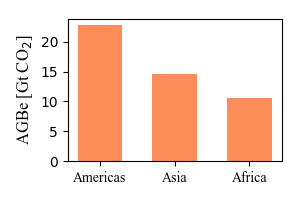
\includegraphics[scale=1]{img/agbe}
%			\caption[Ecosystem service values]{}
%			\label{fig:agbe}
%		\end{figure}
%		\begin{figure}[ht]
%			\centering
%			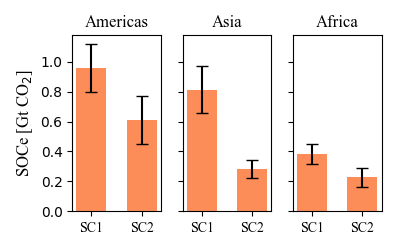
\includegraphics[scale=1]{img/soce}
%			\caption[Ecosystem service values]{}
%			\label{fig:soce}
%		\end{figure}
%
%		\begin{table}[ht]
%			\centering
%			\caption[Soil organic carbon emissions]{Soil organic carbon emissions}
%			\label{tab:soce_tab}
%			\begin{tabular}{lrrrrrrrrr}
%				\hline
%				\multirow{3}{*}{Region} & \multicolumn{3}{c}{SC1}& \multicolumn{3}{c}{SC2} & \multicolumn{3}{c}{SC3} \\
%				& \multicolumn{3}{c}{[Gt CO$_2$]}& \multicolumn{3}{c}{[Gt CO$_2$]} & \multicolumn{3}{c}{[Gt CO$_2$]} \\
%				& min & mean & max & min & mean & max & min & mean & max \\\hline
%				Americas & 0.80 & 0.96 & 1.12 & 0.45 & 0.61 & 0.77 & 0.43 & 0.59 & 0.76 \\
%				Asia & 0.66 & 0.81 & 0.97 & 0.22 & 0.28 & 0.34 & 0.22 & 0.28 & 0.33 \\
%				Africa & 0.32 & 0.39 & 0.45 & 0.17 & 0.23 & 0.29 & 0.16 & 0.23 & 0.29 \\\hline
%			\end{tabular}
%		\end{table}